\chapter{Resultados y discusión}
\label{ch:resultados}

%\avisoLocalizacionArchivo 

\begin{comment}
Escribe en este capítulo los resultados del proyecto.  Este capítulo debería explicar los resultados de forma global, no los resultados de cada fase o iteración.  Probablemente será el capítulo con más tablas y gráficas.  Revisa las secciones~\ref{sec:figuras} y~\ref{sec:tablas} para aprender cómo se escriben en \LaTeX{}.

Tus contribuciones no tienen por qué limitarse al trabajo sistemático del TFG.  Puede que hayas contribuido en aspectos metodológicos, en ideas novedosas, en la planificación de experimentos, en desarrollos matemáticos. Este capítulo está para agrupar todo eso.  Describe con claridad todo lo que ha supuesto contribuciones originales por tu parte.

\warning{Es importante destacar que un resultado negativo es también un resultado.  Es posible que el proyecto planteara abordar un problema con un método que ha demostrado ser no apto.  Si el trabajo ha sido sistemático sigue teniendo mucho valor, puesto que excluye el método para cualquier otro trabajo futuro.  Escribe este tipo de resultados con especial cuidado para destacar que el trabajo se ha realizado de manera sistemática.}
\end{comment}

Este capítulo presenta los resultados globales del trabajo. El proyecto ha producido un sistema de simulación astrodinámica cuyo núcleo es un modelo atmosférico por capas de nueve cuerpos del Sistema Solar y un propagador orbital realista que incorpora el achatamiento planetario ($J_2$) y el arrastre atmosférico. Dado que la validación cuantitativa frente a fuentes primarias ha sido el criterio rector de todo el desarrollo, los resultados se organizan en torno a cuatro ejes. El primero es el modelo atmosférico (Sección~\ref{sec:res-atmosfera}) y su contraste con datos de misiones espaciales (Sección~\ref{sec:res-validacion}), que constituye el resultado central. El segundo es el comportamiento del propagador orbital y su verificación (Sección~\ref{sec:res-propagador}). El tercero es el rendimiento de los agentes y la evaluación de la capa de orquestación (Sección~\ref{sec:res-ia}). El cuarto recoge las  contribuciones originales ---metodológicas y de criterio--- surgidas a lo largo del trabajo (Sección~\ref{sec:res-contribuciones}).

\section{Modelo atmosférico de los nueve cuerpos}
\label{sec:res-atmosfera}

El modelo atmosférico desarrollado cubre los nueve cuerpos considerados. Siete de ellos poseen atmósfera ---la Tierra, Marte, Venus y los cuatro gigantes gaseosos (Júpiter, Saturno, Urano y Neptuno)--- y se describen mediante el perfil \textit{piecewise} exponencial por capas presentado en la Sección~\ref{sec:hidrostatica}. Los otros dos, la Luna y Mercurio, carecen de atmósfera apreciable a efectos orbitales, por lo que solo se les aplica la gravedad central y el achatamiento $J_2$. La altura de referencia $h=0$ se toma en la superficie para los cuerpos rocosos y en el nivel de presión de 1~bar para los gaseosos, que no poseen una superficie sólida definida. La Tabla~\ref{tab:res-atmosfera} resume la configuración de cada cuerpo.

\begin{table}[htbp]
  \centering
  \caption{Configuración del modelo atmosférico por cuerpo}
  \label{tab:res-atmosfera}
  % Definimos que la tabla ocupe exactamente el \textwidth
  % Cambiamos la última columna 'l' por 'X' para que el texto salte de línea si es necesario
  \begin{tabularx}{\textwidth}{l c c c c X}
    \hline
    \textbf{Cuerpo} & \textbf{Capas} & \textbf{Altitud (km)} & \textbf{$\rho(h{=}0)$} & \textbf{$h=0$} & \textbf{Fuente principal} \\
    \hline
    Venus    & 4  & 0--200  & $67$                 & superficie & \gls{VIRA} + cálculo propio \\
    Tierra   & 10 & 0--500  & $1{,}225$            & superficie & \gls{USSA}-76 \\
    Marte    & 7  & 0--300  & $1{,}5\times10^{-2}$ & superficie & Mars Climate Database \\
    Júpiter  & 5  & 0--1000 & $0{,}16$             & 1 bar      & Galileo Probe \\
    Saturno  & 8  & 0--2200 & $0{,}19$             & 1 bar      & Cassini \\
    Urano    & 7  & 0--6500 & $0{,}42$             & 1 bar      & Voyager 2 \\
    Neptuno  & 7  & 0--4000 & $0{,}45$             & 1 bar      & Voyager 2 \\
    \hline
    Mercurio & --- & --- & --- & superficie & sin atmósfera (solo $J_2$) \\
    Luna     & --- & --- & --- & superficie & sin atmósfera (solo $J_2$) \\
    \hline
  \end{tabularx}
\end{table}

El conjunto suma 48 capas exponenciales repartidas entre los siete cuerpos con atmósfera, lo que da lugar a 41 fronteras internas entre capas. En todas ellas la densidad se mantiene continua con un error inferior al 1\,\% ---de hecho, por debajo del 0{,}4\,\% en el peor caso (Marte) y del 0{,}01\,\% en el resto---, gracias a que las alturas de escala $H$ no se fijan a mano, sino que se derivan de la condición de continuidad~\eqref{eq:continuidad}. El modelo abarca un rango de densidades extraordinario, desde los $67~\mathrm{kg\,m^{-3}}$ de la densa troposfera de Venus hasta valores del orden de $10^{-14}~\mathrm{kg\,m^{-3}}$ en las exosferas ---unos quince órdenes de magnitud---, y una extensión vertical que va desde unos pocos cientos de kilómetros en los cuerpos rocosos hasta varios miles en los gigantes (Figura~\ref{fig:perfil-densidad}).

\section{Validación frente a datos de misión}
\label{sec:res-validacion}

La validación cuantitativa del modelo atmosférico constituye el resultado central del trabajo, y se centra en los cuatro gigantes gaseosos, cuyo modelo se calibró a partir de fuentes primarias. La Tierra, Marte y Venus adoptan directamente atmósferas de referencia consolidadas (\gls{USSA}-76, el \textit{Mars Climate Database}~\cite{mcd} y \gls{VIRA}, respectivamente), por lo que no requieren una validación independiente; la Luna y Mercurio carecen de atmósfera. El grado de acuerdo se cuantifica mediante el factor de desviación: el cociente entre la densidad del modelo y la de referencia en cada altitud, tomado siempre como un valor mayor o igual que la unidad, de modo que un factor de 1 indica acuerdo perfecto y un factor de 2, una discrepancia de un factor dos en cualquier sentido. Dos cuerpos, Júpiter y Saturno, disponen de medidas in-situ directas en el archivo \gls{NASA}-\gls{PDS}; para Urano y Neptuno, que carecen de ellas, la referencia es una reconstrucción del perfil de densidad a partir de los datos de \textit{Voyager}~2, cuyo método se detalla en la Sección~\ref{sec:res-contribuciones}. La Tabla~\ref{tab:res-factores} resume los resultados.

 El factor de desviación mediano se calcula sobre todos los puntos de comparación; un valor de 1 indica acuerdo perfecto. Júpiter y Saturno se contrastan con datos in-situ; Urano y Neptuno, con la reconstrucción hidrostática del perfil de \textit{Voyager}~2.

\begin{table}[htbp]
  \centering
  \caption{Resumen de la validación atmosférica.}
  \label{tab:res-factores}
  % Definimos el ancho total y cambiamos la segunda columna 'l' por 'X'
  \begin{tabularx}{\textwidth}{l X c c}
    \hline
    \textbf{Cuerpo} & \textbf{Referencia de validación} & \textbf{Factor mediano} & \textbf{Acuerdo} \\
    \hline
    Júpiter & Galileo Probe, in-situ (431 ptos.)        & $1{,}32$ & $<2\times$ \\
    Saturno & Cassini Grand Finale, in-situ (763 ptos.) & $1{,}06$ & $<2\times$ \\
    Urano   & Voyager 2 reconstruido (hidrostática)     & $1{,}15$ & ---        \\
    Neptuno & Voyager 2 reconstruido + Neptune-\gls{GRAM}     & $1{,}2$  & ---        \\
    \hline
  \end{tabularx}
\end{table}

En conjunto, el modelo reproduce las densidades de referencia dentro de un factor~2 en los cuatro cuerpos, un acuerdo notable si se tiene en cuenta que abarca varios órdenes de magnitud en densidad. A continuación se detalla cada caso.

\subsection{Júpiter: contraste con la sonda Galileo}
\label{sec:res-jupiter}

La atmósfera de Júpiter se ha validado frente a los datos in-situ del instrumento \gls{ASI} de la sonda Galileo, disponibles en el archivo \gls{NASA} \gls{PDS}~\cite{seiff1998,galileoPDS}. De los 693 puntos registrados durante el descenso, la comparación emplea los 431 situados por encima del nivel de referencia de 1~bar ($h\geq 0$); los restantes corresponden a niveles más profundos (presiones mayores que 1~bar), fuera del dominio del modelo.

Sobre esos 431 puntos, el modelo ---recalibrado con los propios datos de Galileo--- reproduce la densidad medida con un factor de desviación mediano de 1,32 (con un valor \gls{RMS}\footnote{El \gls{RMS} (\textit{root mean square}, raíz cuadrática media de las desviaciones) pondera más las desviaciones grandes que la mediana, por lo que recoge mejor la dispersión global del conjunto; es siempre mayor o igual que la mediana.} de 1,45), y el acuerdo se mantiene dentro de un factor 2 en todo el rango de altitudes, desde el nivel de 1~bar hasta más de 1000~km como se ve en las Figuras~\ref{fig:val-jupiter-perfil} y~\ref{fig:val-jupiter-ratio}. La versión inicial del modelo, construida sobre valores de una fuente no contrastada, llegaba a desviarse un factor de hasta 2500 de estas mismas medidas; ese episodio se recoge como lección metodológica en la Sección~\ref{sec:res-contribuciones}.

\begin{figure}[!htbp]
  \centering
  
\includegraphics[width=0.82\textwidth]{tex/imagenes/validacion_jupiter_perfil.png}
  \caption{Perfil de densidad de Júpiter en escala logarítmica. Elaboración propia.}
  \label{fig:val-jupiter-perfil}
\end{figure}

\begin{figure}[!htbp]
  \centering
  
\includegraphics[width=0.82\textwidth]{tex/imagenes/validacion_jupiter_ratio.png}
  \caption{Cociente entre la densidad del modelo y la medida por Galileo en función de la altitud. Elaboración propia.}
  \label{fig:val-jupiter-ratio}
\end{figure}

%\clearpage   % vacía la cola de flotantes (evita "Too many unprocessed floats")

\subsection{Saturno: contraste con Cassini (Grand Finale)}
\label{sec:res-saturno}

La validación de Saturno se ha realizado frente a los datos in-situ obtenidos por la sonda \textit{Cassini} durante su \textit{Grand Finale} de 2017, cuando atravesó repetidamente la alta atmósfera del planeta antes de su entrada final. El conjunto, de 763 puntos, está disponible en el archivo \gls{NASA} \gls{PDS}~\cite{koskinen2021,cassiniPDS}.

El modelo reproduce la mediana de las medidas con un factor de desviación mediano de 1,056; dicho de otro modo, la densidad del modelo se aparta de la mediana de \textit{Cassini} tan solo un 5,6\,\% (el factor y el porcentaje expresan lo mismo: un factor de $1{,}056$ equivale a una diferencia del 5,6\,\%). Además, todos los rangos de altitud quedan dentro de un factor~2 respecto a esa mediana apreciándose en las Figuras~\ref{fig:val-saturno-perfil} y~\ref{fig:val-saturno-ratio}.

\begin{figure}[htbp]
  \centering
  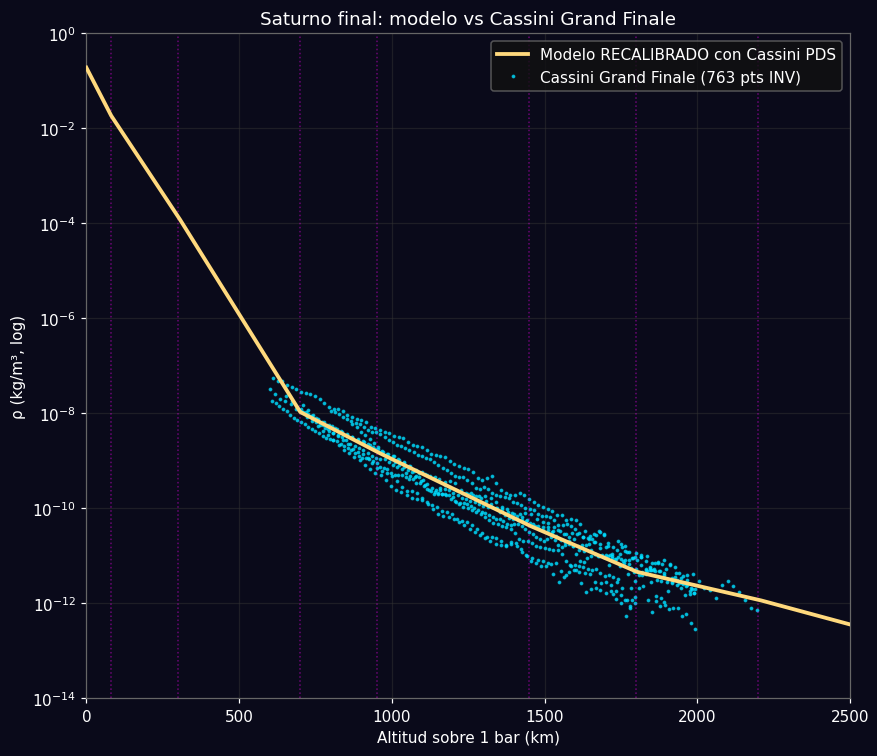
\includegraphics[width=0.82\textwidth]{tex/imagenes/validacion_saturno_perfil.png}
  \caption{Perfil de densidad de Saturno. Elaboración propia.}
  \label{fig:val-saturno-perfil}
\end{figure}

\begin{figure}[htbp]
  \centering
  
\includegraphics[width=0.82\textwidth]{tex/imagenes/validacion_saturno_ratio.png}
  \caption{Cociente modelo/\textit{Cassini} frente a la altitud. Elaboración propia.}
  \label{fig:val-saturno-ratio}
\end{figure}

La dispersión de la Figura ~\ref{fig:val-saturno-ratio} corresponde a la variabilidad latitudinal real como se aprecia en la Figura~\ref{fig:val-saturno-lat-perfil} ya que la densidad a una altitud dada varía con la latitud, y el modelo (línea blanca) sigue la mediana latitudinal.

A diferencia de Júpiter, las medidas de \textit{Cassini} presentan una dispersión  considerable (su valor \gls{RMS} ronda un factor~2). Esta dispersión, sin embargo, no es un error del modelo: refleja un fenómeno físico real. La atmósfera de Saturno no es igual en todas partes; a una misma altitud, su densidad cambia de forma apreciable según la latitud, de modo análogo a como en la Tierra la atmósfera difiere entre el ecuador y los polos. Como \textit{Cassini} muestreó un amplio rango de latitudes (de $-85^\circ$ a $+80^\circ$), a cada altitud no le corresponde un único valor de densidad, sino todo un abanico de valores; de ahí la anchura de la nube de puntos.

Un modelo unidimensional como el desarrollado no puede depender de la latitud, así que adopta en cada altitud la mediana de todas ellas (la línea central de ese abanico). Y esta es justamente la elección adecuada para calcular el arrastre orbital: a lo largo de una órbita el satélite recorre muchas latitudes distintas, por lo que el frenado efectivo depende de la densidad promediada sobre ellas, no de la de una latitud concreta. La Figura~\ref{fig:val-saturno-lat-perfil} muestra las medidas separadas por bandas de latitud, y la Figura~\ref{fig:val-saturno-lat-banda} confirma que el modelo permanece dentro de la banda intercuartílica ---el rango central que abarca la mitad de las latitudes--- en todo el intervalo.

\begin{figure}[htbp]
  \centering
  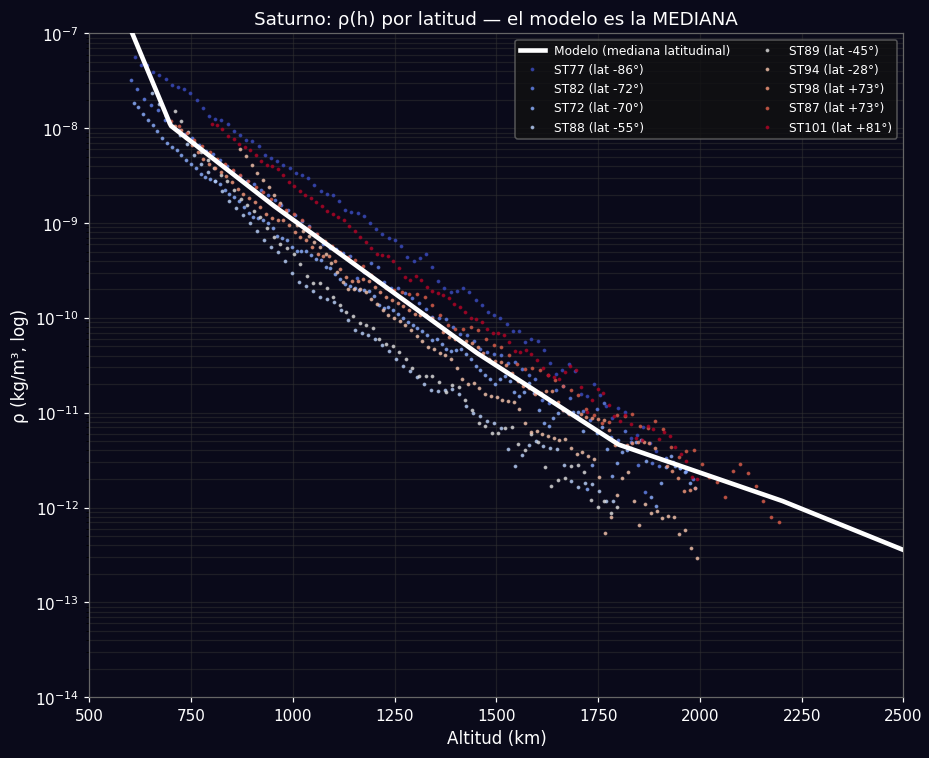
\includegraphics[width=0.82\textwidth]{tex/imagenes/validacion_saturno_lat_perfil.png}
  \caption{Medidas de \textit{Cassini} desglosadas por bandas de latitud (entre $-85^\circ$ y $+80^\circ$). Elaboración propia.}
  \label{fig:val-saturno-lat-perfil}
\end{figure}

\begin{figure}[htbp]
  \centering
  
\includegraphics[width=0.82\textwidth]{tex/imagenes/validacion_saturno_lat_banda.png}
  \caption{Modelo frente a la mediana de \textit{Cassini} por intervalos de altitud, con su banda intercuartílica (percentiles 25--75\,\%). Elaboración propia.}
  \label{fig:val-saturno-lat-banda}
\end{figure}


\subsection{Urano y Neptuno: contraste con Voyager 2 reconstruido}
\label{sec:res-urano-neptuno}

A diferencia de Júpiter y Saturno, ni Urano ni Neptuno disponen de medidas de densidad in-situ: cada uno fue visitado una sola vez por la \textit{Voyager}~2 (en 1986 y 1989, respectivamente), que midió perfiles de temperatura y presión, pero no de densidad. Para poder validar el modelo se reconstruyó el perfil de densidad a partir de esos datos mediante integración hidrostática ---el mismo procedimiento que emplean los modelos de referencia \gls{GRAM} de la \gls{NASA}---, y se contrastó de forma cruzada con dichos modelos~\cite{uranusGRAM2021,neptuneGRAM2020}, con acuerdos inferiores al 2\,\%. Por tratarse de una aportación metodológica propia, el método se detalla en la Sección~\ref{sec:res-contribuciones}.

\textbf{Urano.} Frente a la reconstrucción de \textit{Voyager}~2~\cite{lindal1987,tyler1986,anderson1987}, el modelo recalibrado alcanza un factor de desviación mediano de 1,15 en el rango 0--262~km cubierto por la sonda, frente al 2,49 del modelo inicial. La mejora provino de añadir una capa intermedia a 150~km, que corrigió una sobreestimación de la estratosfera (Figuras~\ref{fig:val-urano-perfil} y~\ref{fig:val-urano-ratio}). El acuerdo es excelente hasta unos 200~km; por encima, cerca del techo del rango validado (262~km), el factor del modelo recalibrado crece hacia 2, lo que refleja la menor densidad de datos de \textit{Voyager} en la alta atmósfera y la transición hacia la termosfera~\cite{melin2020}, ya extrapolada. Las capas superiores del modelo son, por tanto, las menos fiables.

\begin{figure}[htbp]
  \centering
  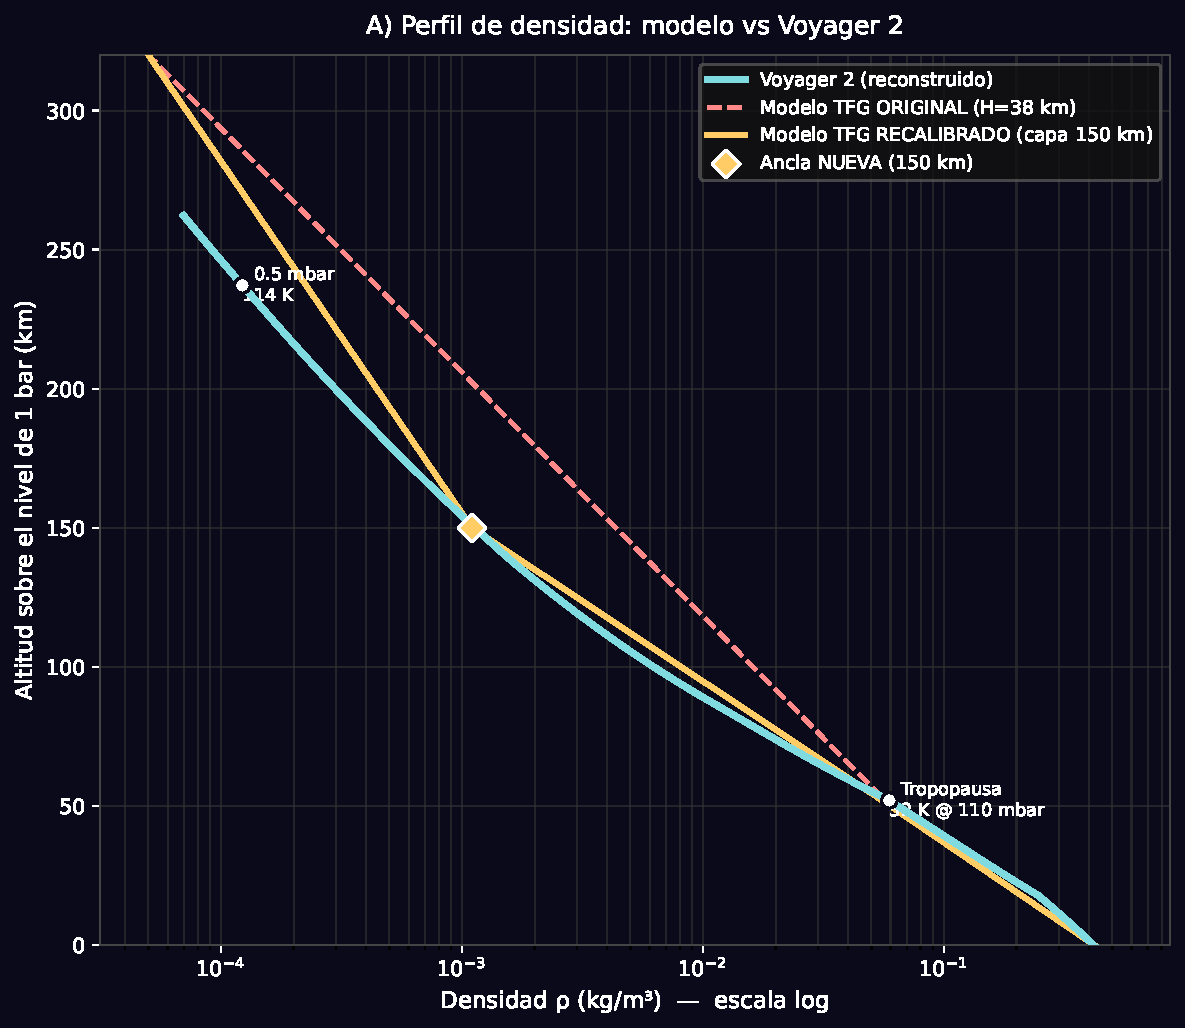
\includegraphics[width=0.82\textwidth]{tex/imagenes/validacion_urano_perfil.pdf}
  \caption{Perfil de densidad de Urano. Elaboración propia.}
  \label{fig:val-urano-perfil}
\end{figure}

\begin{figure}[htbp]
  \centering
  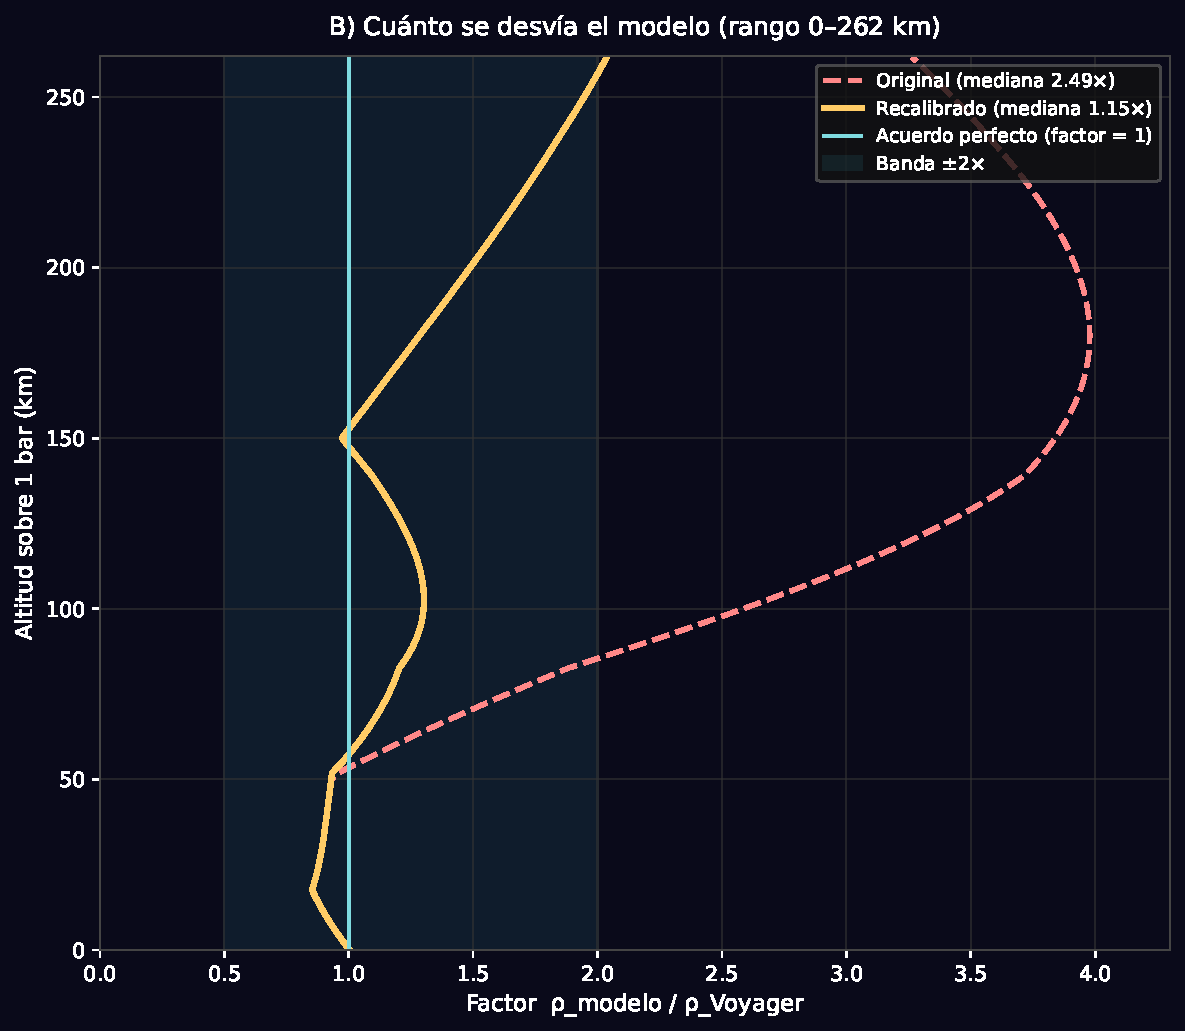
\includegraphics[width=0.82\textwidth]{tex/imagenes/validacion_urano_ratio.pdf}
  \caption{Factor de desviación del modelo de Urano respecto a \textit{Voyager}~2 en función de la altitud. Elaboración propia.}
  \label{fig:val-urano-ratio}
\end{figure}

\textbf{Neptuno.} El caso de Neptuno fue más extremo. Validado contra la reconstrucción de \textit{Voyager}~2~\cite{lindal1990,lindal1992} y los puntos del modelo Neptune-\gls{GRAM}~\cite{neptuneGRAM2020}, el modelo recalibrado logra un factor de desviación típico de 1,2, frente al 8,0 del modelo inicial. Este último subestimaba la densidad hasta en un factor de 100 entre 20 y 300~km de altitud (Figura~\ref{fig:val-neptuno-perfil}, curva discontinua), un error grave que la validación permitió detectar y corregir, y que se describe en detalle como aportación en la Sección~\ref{sec:res-contribuciones} (Figuras~\ref{fig:val-neptuno-perfil} y~\ref{fig:val-neptuno-ratio}).

\begin{figure}[htbp]
  \centering
  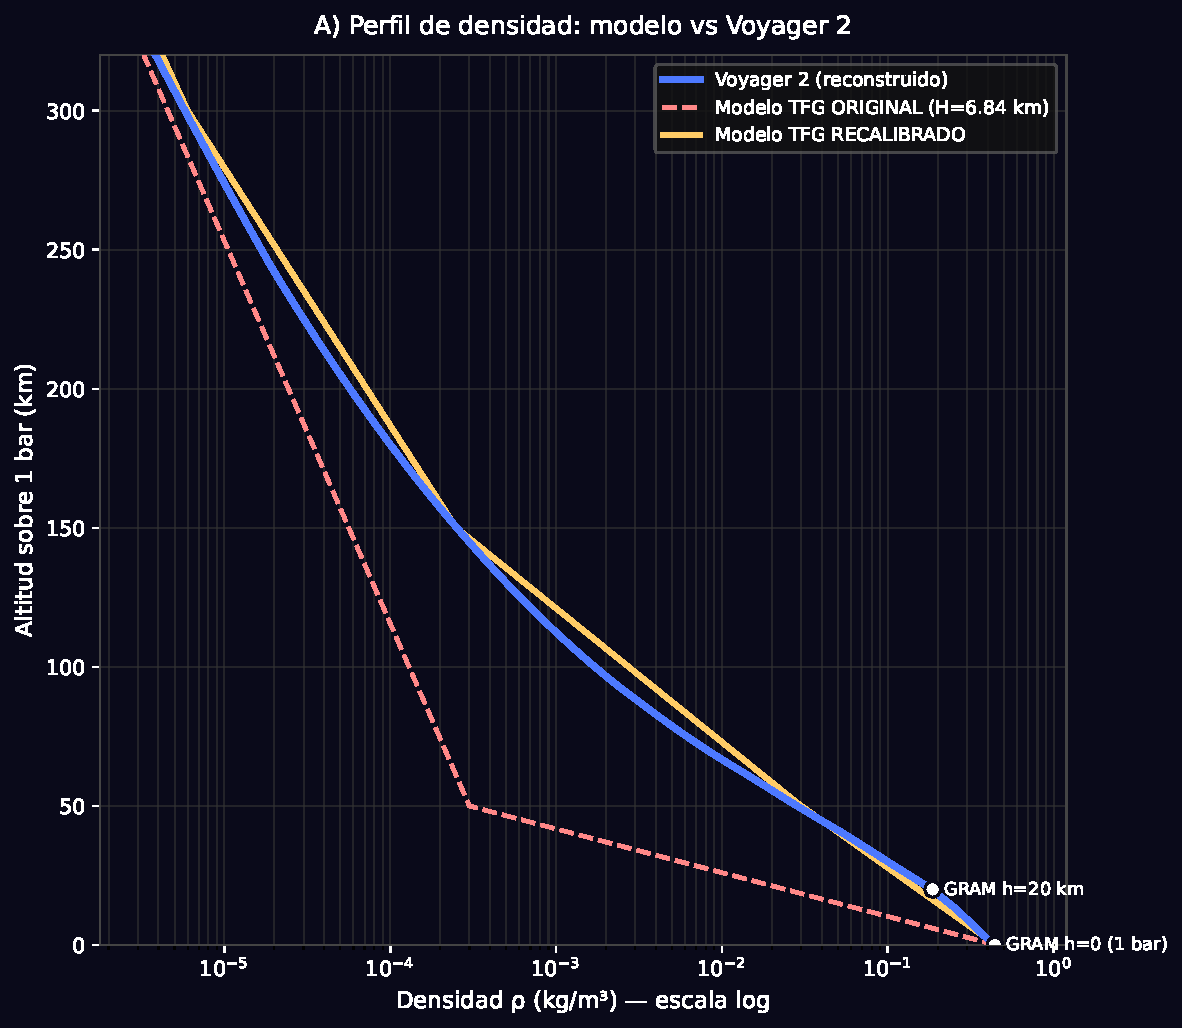
\includegraphics[width=0.82\textwidth]{tex/imagenes/validacion_neptuno_perfil.pdf}
  \caption{Perfil de densidad de Neptuno. Elaboración propia.}
  \label{fig:val-neptuno-perfil}
\end{figure}

\begin{figure}[htbp]
  \centering
  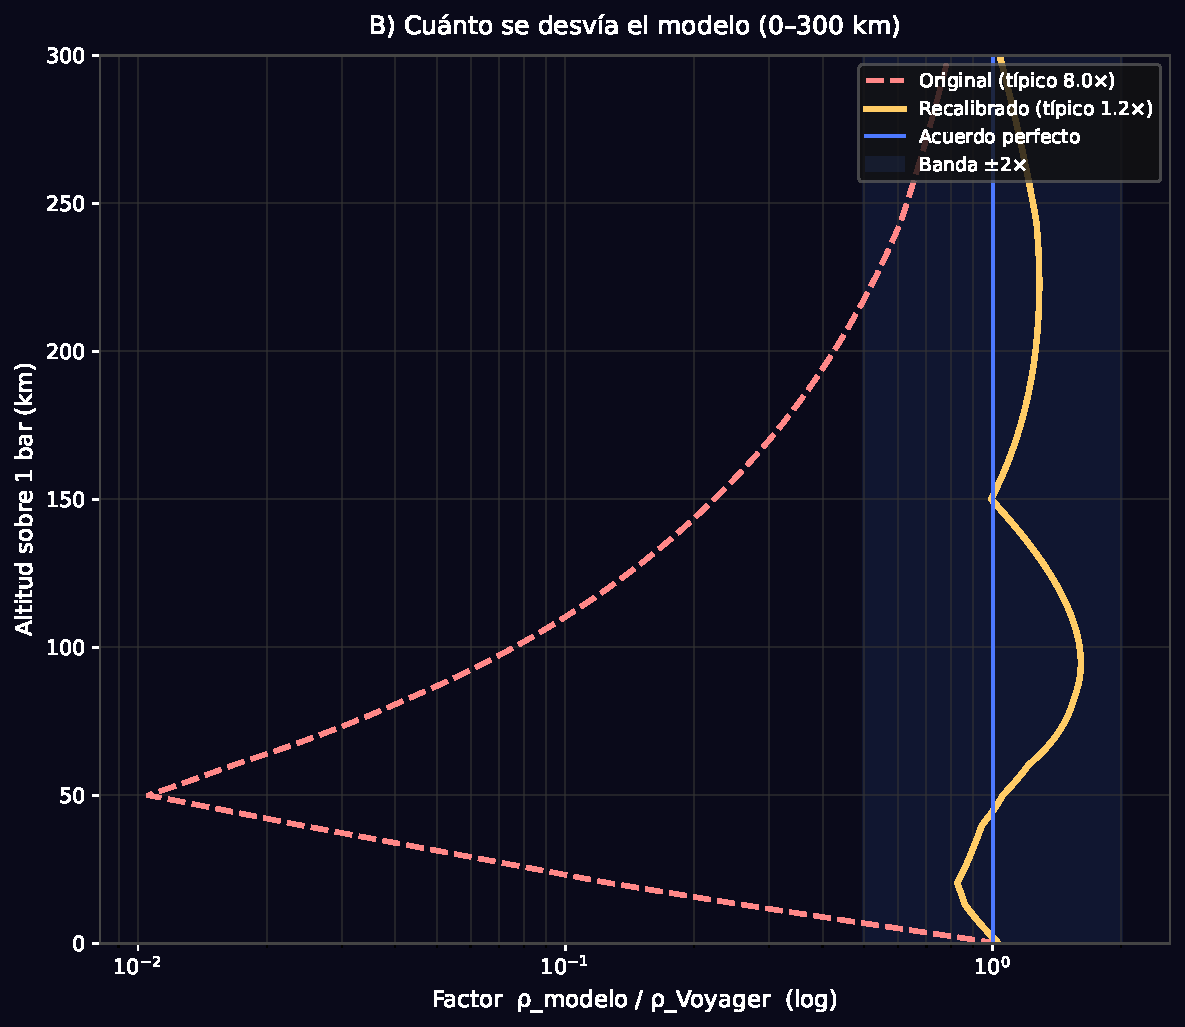
\includegraphics[width=0.82\textwidth]{tex/imagenes/validacion_neptuno_ratio.pdf}
  \caption{Factor de desviación del modelo de Neptuno respecto a \textit{Voyager}~2. Elaboración propia.}
  \label{fig:val-neptuno-ratio}
\end{figure}



\section{Comportamiento del propagador orbital}
\label{sec:res-propagador}

El propagador realista (gravedad central $+\,J_2+$ arrastre, integrado con el método de Cowell) se ha ejercitado sobre los nueve cuerpos para comprobar que su comportamiento es físicamente correcto y numéricamente robusto en todo el catálogo, y no solo en la Tierra.

Efectos combinados de $J_2$ y arrastre. La Figura~\ref{fig:efectos-j2drag} (Capítulo~\ref{ch:desarrollo}) ilustra el caso de referencia, una órbita tipo \gls{ISS}: el propagador reproduce simultáneamente las dos firmas esperadas ---las oscilaciones periódicas de período corto inducidas por $J_2$ (el ``dentado'' de la altitud) y el descenso secular causado por el arrastre---, además de la regresión nodal. Esta última se contrastó cuantitativamente con la teoría de Brouwer en la Sección~\ref{sec:brouwer}, con un acuerdo inferior al 1\,\% en los casos de $J_2$ moderado.

Detección automática de reentrada. El propagador incorpora un criterio de reentrada que se activa cuando la altitud cruza por debajo del umbral propio de cada cuerpo, o cuando el integrador no puede continuar. El comportamiento es el esperado en todo el catálogo: las órbitas bajas de los cuerpos con atmósfera decaen y reentran, mientras que la Luna y Mercurio, sin atmósfera, mantienen una órbita estable gobernada únicamente por $J_2$.

Suite de verificación automática. Para asegurar que el propagador no se rompe ni produce resultados espurios en ningún cuerpo, se desarrolló una batería de pruebas automáticas que recorre los nueve cuerpos aplicando seis comprobaciones a cada uno (54 en total). La Tabla~\ref{tab:res-tests} las resume; las 54 se superan en la versión actual del código.

\begin{table}[htbp]
  \centering
  \caption{Comprobaciones de la verificación automática del propagador.}
  \label{tab:res-tests}
  \begin{tabular}{l p{8.2cm}}
    \hline
    \textbf{Comprobación} & \textbf{Qué verifica} \\
    \hline
    Radio del cuerpo         & Coincide con el valor de \texttt{poliastro} \\
    Densidad atmosférica     & Finita y monótona (o nula si el cuerpo no tiene atmósfera) \\
    Órbita kepleriana ideal  & Altitud constante en ausencia de perturbaciones \\
    Propagación perturbada   & Se ejecuta sin fallos numéricos y con valores finitos \\
    Órbita alta              & Permanece acotada (no diverge) \\
    Órbita baja              & Decae o reentra con arrastre; estable solo con $J_2$ si no hay atmósfera \\
    \hline
  \end{tabular}
\end{table}

Una limitación documentada. En los planetas de $J_2$ muy elevado (Júpiter y Saturno), las órbitas muy bajas (a unos pocos miles de kilómetros sobre la superficie) resultan inviables: la fuerte oscilación de los elementos osculadores por $J_2$ hunde momentáneamente el perigeo bajo la superficie, y el integrador se detiene y etiqueta el caso como reentrada. No es un fallo del propagador, sino el reflejo de que esas órbitas no son físicamente sostenibles; el fenómeno se identificó, se acotó y se documentó.

\section{Resultados de los agentes de RL}
\label{sec:res-ia}

Esta sección presenta el comportamiento de los agentes de aprendizaje por refuerzo desarrollados en la Sección~\ref{sec:ia}, evaluados frente a sus respectivos jueces. Todos los resultados se obtienen ejecutando los agentes ya entrenados sobre el modelo físico validado: las figuras no contienen datos sintéticos, sino la respuesta real de
cada agente.

\subsection{Evaluación estadística de los agentes}
\label{sec:res-ia-stats}

Antes de examinar el comportamiento de cada agente por separado, conviene fundamentar los resultados sobre una base estadística. Para ello, cada agente se ha evaluado sobre cincuenta episodios independientes generados con escenarios aleatorios; en los agentes con un especialista por planeta (aerofrenado y mantenimiento), son cincuenta episodios por cuerpo, esto es, trescientos cincuenta en total. Las semillas de evaluación se han tomado en un rango disjunto del empleado durante el entrenamiento, de modo que los escenarios de prueba sean efectivamente no vistos; la política se consulta de forma determinista, por lo que los valores son reproducibles. De cada episodio se registran las métricas relevantes ---exceso de $\Delta v$ respecto al óptimo, error de llegada, número de pasadas, presión dinámica máxima soportada y resultado del episodio--- y se resumen mediante su media y su desviación típica.

La Tabla~\ref{tab:res-ia-estadistica} recoge los tres agentes de maniobra impulsiva. El agente de transferencia \gls{LEO}$\rightarrow$\gls{GEO} opera sobre un escenario fijo y alcanza el óptimo de forma prácticamente exacta. Los agentes generales ---transferencias coplanares y cambio de plano--- se evalúan sobre el rango útil de operación y mantienen el exceso medio de $\Delta v$ por debajo del 1\,\% y el error de llegada en torno al 1\,\%, con una tasa de éxito del 92\,\%. El agente de cambio de plano, además, alcanza la inclinación pedida con un error medio de solo $0{,}12 \pm 0{,}10$ grados.

\begin{table}[htbp]
  \centering
  \caption{Evaluación estadística de los agentes de maniobra impulsiva sobre escenarios de evaluación independientes ($N$ episodios).}
  \label{tab:res-ia-estadistica}
  \begin{tabularx}{\textwidth}{X c c c c}
    \hline
    \textbf{Agente} & \textbf{$N$} & \textbf{Tasa de éxito} & \textbf{Exceso de $\Delta v$} & \textbf{Error de llegada} \\
    \hline
    Transferencia LEO$\rightarrow$GEO      & 1  & ---     & $-0{,}03$\,\%              & $0{,}08$\,\%              \\
    Transferencias coplanares generales    & 50 & $46/50$ & $-0{,}72 \pm 5{,}04$\,\%   & $0{,}99 \pm 0{,}65$\,\%   \\
    Cambio de plano (tridimensional)       & 50 & $46/50$ & $+1{,}00 \pm 0{,}74$\,\%   & $1{,}44 \pm 0{,}81$\,\%   \\
    \hline
  \end{tabularx}
\end{table}

El exceso de $\Delta v$ presenta valores medios ligeramente negativos en las transferencias coplanares: no significan que el agente supere al óptimo de Hohmann, sino que sacrifica una fracción mínima de precisión de llegada a cambio de un coste algo menor, un compromiso admitido por la función de recompensa. Fuera del rango útil, en las bajadas muy profundas (razón de radios inferior a $0{,}2$, que corresponden a divisiones a menos de un quinto del radio inicial), el error de llegada crece hasta el orden del 6\,\%: es una limitación conocida del agente coplanar, poco relevante en la práctica porque esas maniobras extremas son precisamente las que resuelve el aerofrenado.

Conviene precisar dónde se sitúan los pocos episodios que no alcanzan el criterio de éxito, pues su naturaleza es reveladora. En el agente coplanar se concentran en los bordes del rango de operación (razones de radios próximas a los extremos, $0{,}2$ y $11$), donde superan el umbral del 2\,\% solo por unas centésimas. En el agente de cambio de plano aparecen en los giros mayores (ángulos próximos al máximo de $40$ grados), con un exceso de $\Delta v$ de entre el 2 y el 3,5\,\%; ahora bien, incluso en esos casos el agente alcanza la inclinación pedida con un error inferior a $0{,}4$ grados. Es decir, no son maniobras que fracasen ---llegan a su destino y a la orientación correctas---, sino maniobras que aterrizan con un coste ligeramente superior al óptimo en las regiones más exigentes del espacio de escenarios. Un impulso de corrección adicional, ajeno a la formulación de un solo paso adoptada aquí, bastaría para absorber ese residuo; se apunta como una extensión inmediata de bajo coste.

Los agentes de aerofrenado y de mantenimiento se evalúan por cuerpo. En el aerofrenado, el resultado es contundente: los siete especialistas completan la maniobra en la totalidad de los trescientos cincuenta episodios (cincuenta por cuerpo), sin una sola destrucción ni un solo episodio con el tiempo agotado. La Tabla~\ref{tab:res-ia-aero-stats} detalla, por cuerpo, el número de pasadas, el $\Delta v$ de ajuste consumido y ---lo más relevante para la seguridad--- la presión dinámica máxima soportada, que en todos los casos se mantiene por debajo del límite de $0{,}6\ \mathrm{N/m^2}$ fijado como criterio. Ese margen confirma que el corredor de perigeo derivado de cada atmósfera es efectivamente seguro.

\begin{table}[htbp]
  \centering
  \caption{Estadística del agente de aerofrenado por cuerpo.}
  \label{tab:res-ia-aero-stats}
  \begin{tabular}{l c c c}
    \hline
    \textbf{Cuerpo} & \textbf{Pasadas} & {\boldmath $\Delta v$} \textbf{de ajuste (m/s)} & {\boldmath $q$}$_{\max}$ \textbf{(N/m}$^{\mathbf{2}}$\textbf{)} \\
    \hline
    Venus   & $232 \pm 66$  & $1{,}75 \pm 0{,}14$  & $0{,}255 \pm 0{,}002$ \\
    Tierra  & $221 \pm 64$  & $2{,}14 \pm 0{,}23$  & $0{,}302 \pm 0{,}010$ \\
    Marte   & $102 \pm 28$  & $0{,}98 \pm 0{,}07$  & $0{,}196 \pm 0{,}000$ \\
    Júpiter & $371 \pm 105$ & $18{,}41 \pm 1{,}69$ & $0{,}405 \pm 0{,}004$ \\
    Saturno & $201 \pm 57$  & $11{,}06 \pm 0{,}90$ & $0{,}265 \pm 0{,}001$ \\
    Urano   & $110 \pm 31$  & $17{,}05 \pm 1{,}19$ & $0{,}158 \pm 0{,}002$ \\
    Neptuno & $140 \pm 39$  & $16{,}92 \pm 1{,}30$ & $0{,}252 \pm 0{,}000$ \\
    \hline
  \end{tabular}
\end{table}

El agente de mantenimiento presenta la misma robustez: conserva la órbita dentro de la banda de tolerancia en los trescientos cincuenta episodios (cincuenta por cuerpo, con altitud e inclinación objetivo sorteadas). La Tabla~\ref{tab:res-ia-keep-stats} resume, por cuerpo, el coste anual de $\Delta v$ del agente frente al de una estrategia ingenua ---un re-\textit{boost} máximo en cuanto la órbita cae a la mitad inferior de la banda--- y el ahorro resultante.

\begin{table}[htbp]
  \centering
  \caption{Estadística del agente de mantenimiento orbital por cuerpo.}
  \label{tab:res-ia-keep-stats}
  \begin{tabular}{l c c c}
    \hline
    \textbf{Cuerpo} & {\boldmath $\Delta v$} \textbf{ agente (m/s·año)} & {\boldmath $\Delta v$} \textbf{ ingenua (m/s·año)} & \textbf{Ahorro} \\
    \hline
    Venus   & $67{,}7 \pm 68{,}8$ & $75{,}7 \pm 80{,}3$   & $10{,}6$\,\%  \\
    Tierra  & $55{,}3 \pm 62{,}4$ & $58{,}5 \pm 70{,}5$   & $5{,}4$\,\%   \\
    Marte   & $65{,}2 \pm 67{,}9$ & $115{,}4 \pm 134{,}7$ & $43{,}5$\,\% \\
    Júpiter & $67{,}7 \pm 68{,}9$ & $68{,}9 \pm 71{,}9$   & $1{,}7$\,\%   \\
    Saturno & $72{,}1 \pm 71{,}8$ & $72{,}7 \pm 73{,}4$   & $0{,}9$\,\%   \\
    Urano   & $57{,}9 \pm 66{,}2$ & $58{,}0 \pm 67{,}2$   & $0{,}1$\,\%   \\
    Neptuno & $67{,}8 \pm 69{,}0$ & $67{,}4 \pm 70{,}4$   & $-0{,}5$\,\% \\
    \hline
  \end{tabular}
\end{table}

El ahorro delata un comportamiento honesto y físicamente esperable: es grande en Marte (un 43\,\%, donde su atmósfera tenue permite estrategias de corrección más finas) pero prácticamente nulo en los gigantes (diferencias por debajo del 2\,\%, dentro del ruido estadístico). En estos últimos, el $\Delta v$ de mantenimiento está casi enteramente fijado por la física ---es la energía que hay que reponer, decida quien lo decida---, de modo que el agente no puede batir a la estrategia ingenua, solo igualarla. El detalle de cómo varía este coste con la altitud se analiza en la Sección~\ref{sec:res-ia-mantenimiento}.

Cabe señalar una limitación metodológica, en aras de la honestidad: cada agente se ha entrenado con una única semilla de entrenamiento, por lo que las cifras anteriores caracterizan el rendimiento del modelo final, no la variabilidad entre distintas inicializaciones del entrenamiento. Repetir el entrenamiento con varias semillas reforzaría aún más la solidez estadística de los resultados y queda como línea de trabajo inmediata.

\subsection{Transferencias impulsivas: precisión e invariancia de escala}
\label{sec:res-ia-transfer}

El primer agente, especializado en la transferencia de una órbita baja a una \gls{GEO} (\gls{LEO}$\rightarrow$\gls{GEO}), aprende la maniobra óptima sin conocer su fórmula: alcanza un coste total de $\Delta v$ que se desvía solo un 0,03\,\% del óptimo de Hohmann~\eqref{eq:hohmann}, y llega a la órbita objetivo con un error inferior al 0,1\,\%. Sobre un caso de solución conocida, este resultado valida que el procedimiento de aprendizaje funciona.

El agente general (adimensional) extiende ese comportamiento a cualquier transferencia coplanaria. La Figura~\ref{fig:ia-dv-r} compara su coste con el óptimo en todo el rango de ratios $R=r_2/r_1$, tanto al subir ($R>1$) como al bajar ($R<1$): el agente reproduce el óptimo en toda la franja. En el rango útil ($R$ entre $0{,}2$ y $11$) el exceso sobre el óptimo se mantiene por debajo del 1\,\%, con un error de llegada inferior al 2\,\%. El agente sube con algo más de precisión que baja ---en las bajadas tiende a quedarse ligeramente corto---, y solo en el extremo de bajadas muy profundas ($R<0{,}2$) la precisión se degrada de forma apreciable.

\begin{figure}[htbp]
  \centering
  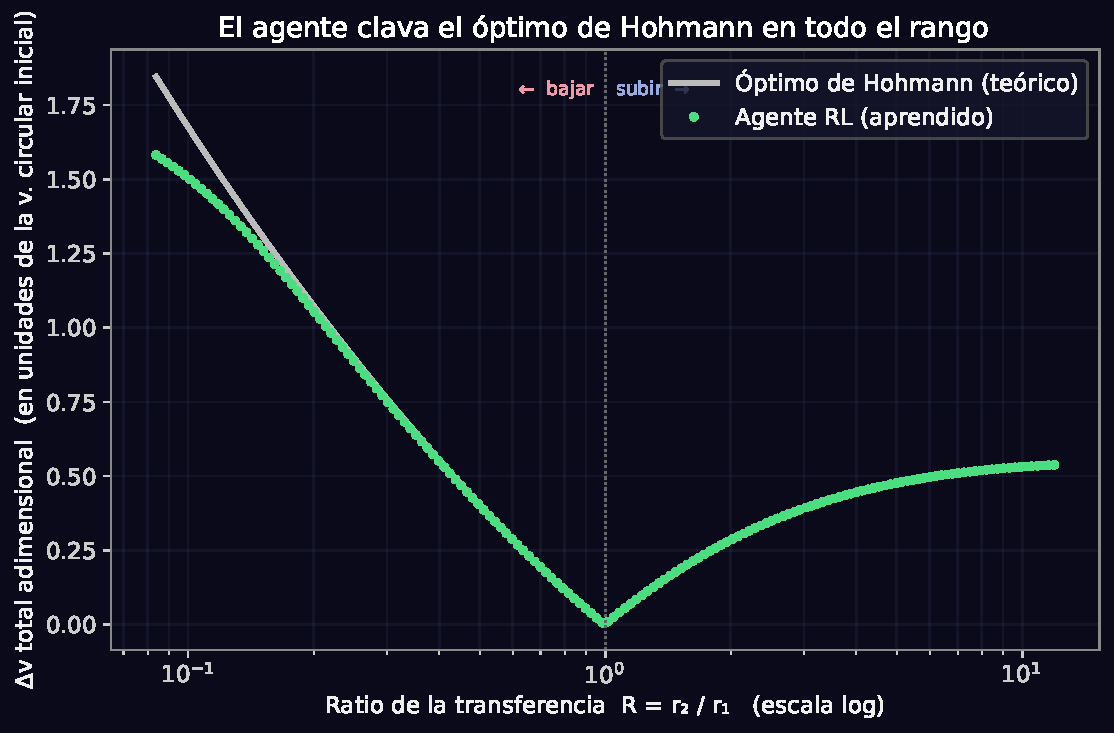
\includegraphics[width=0.82\textwidth]{tex/imagenes/ia_transfer_dv_vs_R.pdf}
  \caption{Coste de la transferencia ($\Delta v$ total) del agente general frente al óptimo de Hohmann. Elaboración propia}
  \label{fig:ia-dv-r}
\end{figure}

La propiedad más relevante de este agente es la invariancia de escala razonada en la Sección~\ref{sec:ia-transfer}. La Figura~\ref{fig:ia-invariancia} muestra el exceso del agente sobre el óptimo cuando la misma política, entrenada una sola vez, se aplica a los nueve cuerpos del estudio sin reentrenamiento alguno. Los puntos de todos los cuerpos se superponen para cada valor de $R$: el resultado no depende del planeta, lo que confirma empíricamente que la maniobra solo depende de la proporción entre órbitas~\eqref{eq:hohmann-adim}. Un único agente sirve, por tanto, para toda transferencia coplanaria en cualquier cuerpo, desde la Tierra hasta Júpiter, la Luna o Mercurio.

\begin{figure}[htbp]
  \centering
  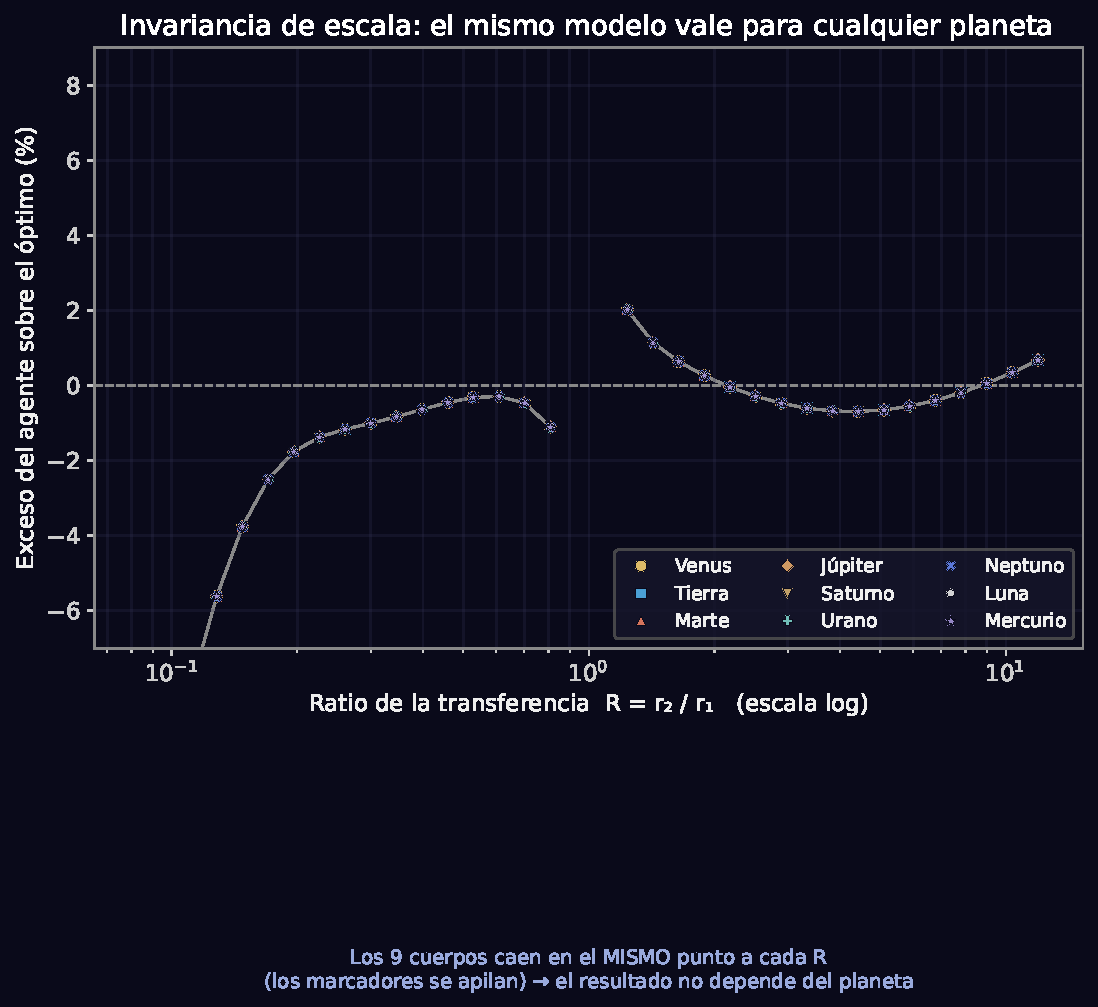
\includegraphics[width=0.82\textwidth]{tex/imagenes/ia_transfer_invariancia.pdf}
  \caption{Exceso del agente sobre el óptimo al aplicar la misma política, sin reentrenar, a los nueve cuerpos. Elaboración propia}
  \label{fig:ia-invariancia}
\end{figure}

A modo de ilustración, la Figura~\ref{fig:ia-orbita-leogeo} representa la transferencia \gls{LEO}$\rightarrow$\gls{GEO} sobre el plano orbital con los impulsos calculados por el agente mientras que en la Figura~\ref{fig:ia-orbita-bajada} se muestra una transferencia de \gls{GEO}$\rightarrow$\gls{LEO} sobre el plano orbital con los impulsos calculados por el agente.

\begin{figure}[htbp]
  \centering
  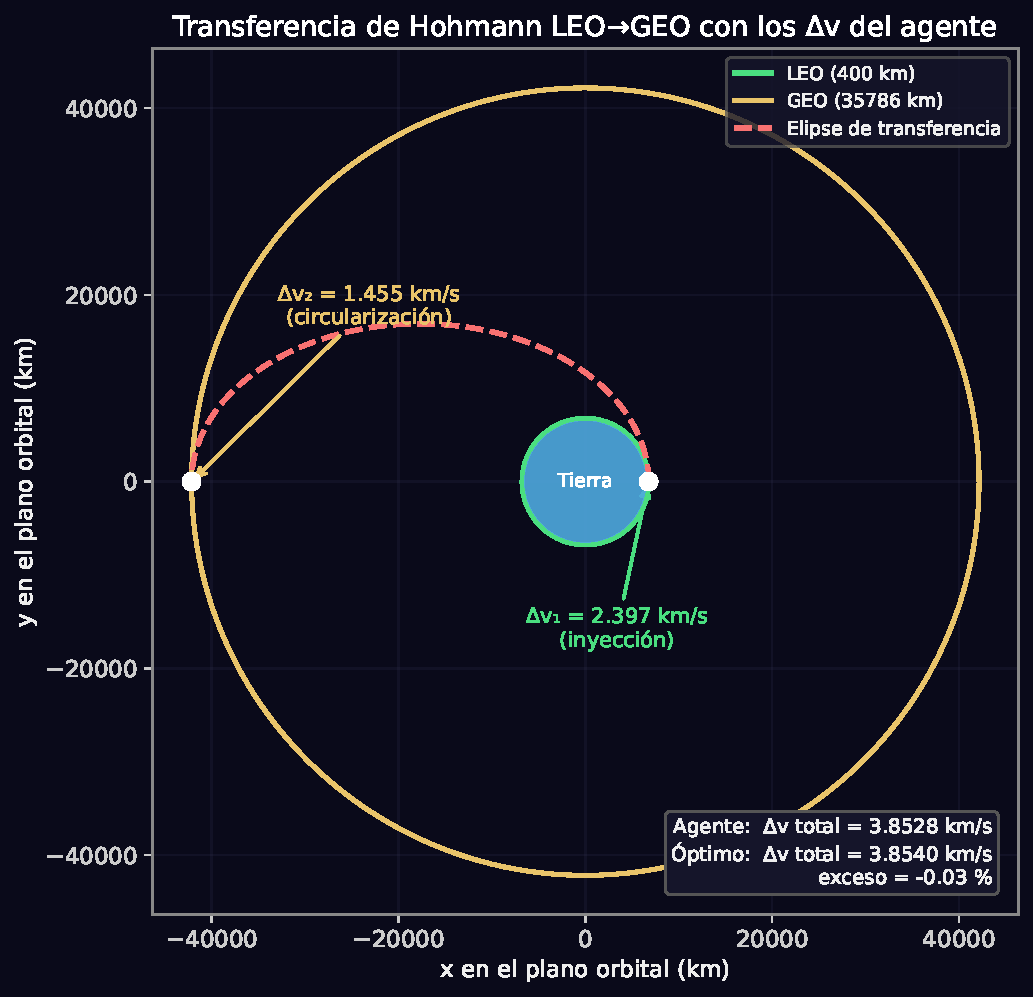
\includegraphics[width=0.62\textwidth]{tex/imagenes/ia_orbita_hohmann_leo_geo.pdf}
  \caption{Transferencia de Hohmann \gls{LEO}$\rightarrow$\gls{GEO} ejecutada con los impulsos del agente. Elaboración propia}
  \label{fig:ia-orbita-leogeo}
\end{figure}

\begin{figure}[htbp]
  \centering
  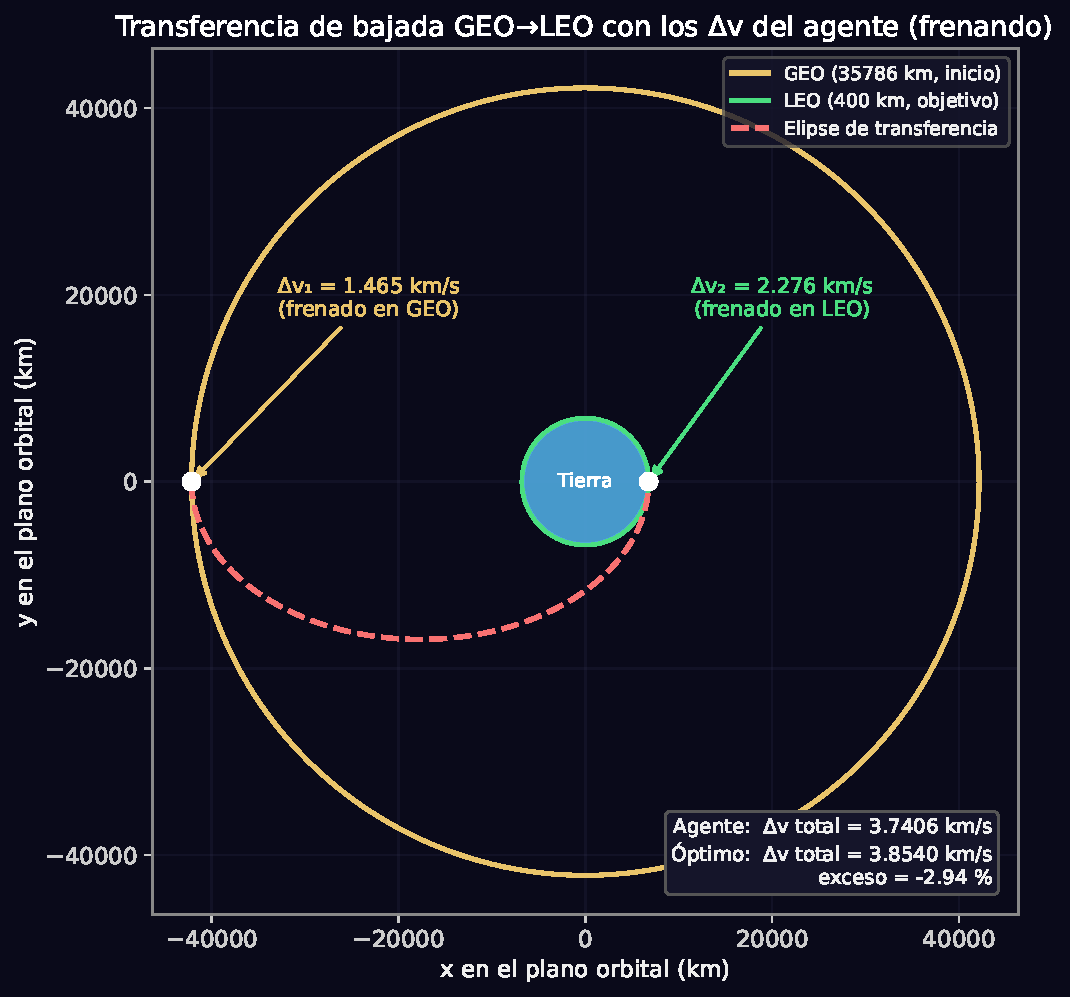
\includegraphics[width=0.62\textwidth]{tex/imagenes/ia_orbita_bajada_geo_leo.pdf}
  \caption{Transferencia de bajada \gls{GEO}$\rightarrow$\gls{LEO} ejecutada con los impulsos del agente; en este caso ambos impulsos son de frenado. Elaboración propia}
  \label{fig:ia-orbita-bajada}
\end{figure}

\subsection{Transferencias con cambio de plano: extensión tridimensional}
\label{sec:res-ia-transfer3d}

La extensión tridimensional del agente de transferencias (Sección~\ref{sec:ia-transfer3d}) resuelve transferencias de subida que incluyen un cambio de plano. Evaluado frente al óptimo de Hohmann con cambio de plano combinado, mantiene un exceso de coste inferior al 2\,\% en todo el rango considerado ---ratios $R$ hasta $11{,}94$ y cambios de plano $\Delta i$ hasta $40^{\circ}$---, alcanzando la órbita objetivo con la inclinación pedida (error inferior a $0{,}3^{\circ}$). La Figura~\ref{fig:ia3d-dv-r} compara su coste con el óptimo para un cambio de plano fijo de $28{,}5^{\circ}$ ---el de una inyección a la órbita geoestacionaria--- en función del ratio: el agente reproduce el óptimo en toda la franja.

\begin{figure}[htbp]
  \centering
  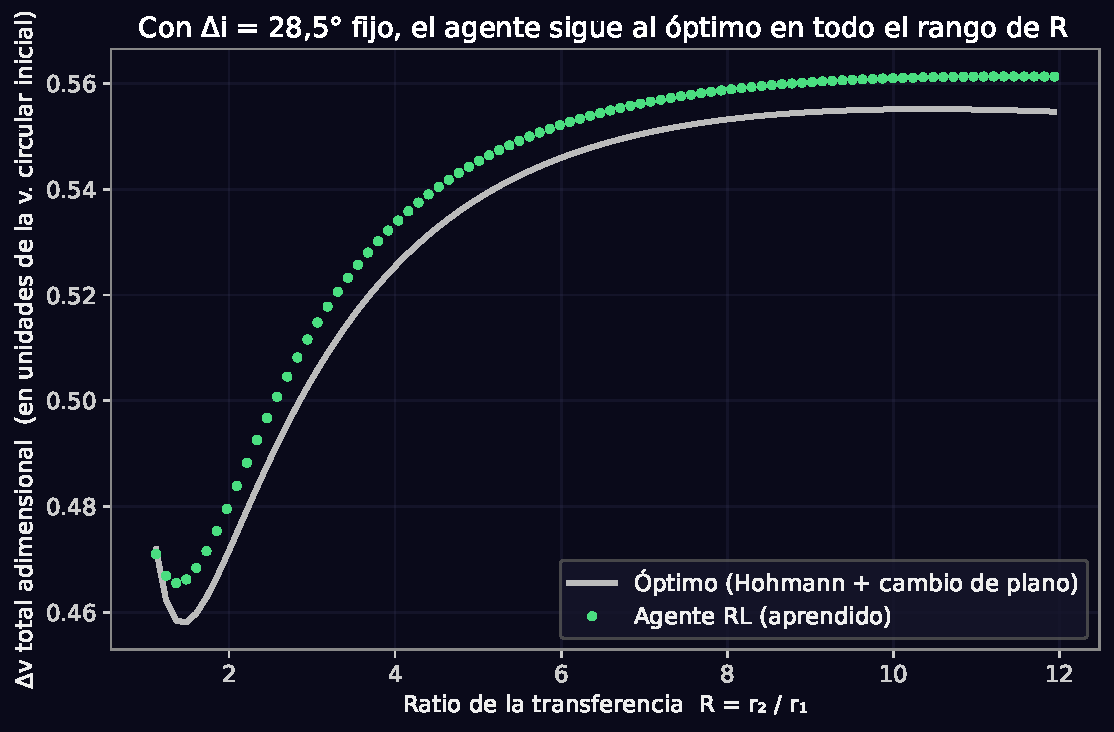
\includegraphics[width=0.82\textwidth]{tex/imagenes/ia_transfer3d_dv_vs_R.pdf}
  \caption{Coste de la transferencia ($\Delta v$ total) del agente tridimensional frente al óptimo de Hohmann con cambio de plano. Elaboración propia.}
  \label{fig:ia3d-dv-r}
\end{figure}

El comportamiento más ilustrativo es el reparto del giro. La Figura~\ref{fig:ia3d-reparto} muestra qué parte del cambio de plano total conviene realizar en cada impulso: la franja del apogeo absorbe casi todo el giro, mientras que la del perigeo es mínima. Para una inyección a la \gls{GEO} ($\Delta i=28{,}5^{\circ}$), el óptimo gira solo unos $2^{\circ}$ en el perigeo y los $26^{\circ}$ restantes en el apogeo. El agente reproduce esta estrategia ---concentra el giro arriba--- sin que se le haya indicado: es consecuencia directa de minimizar el coste del giro (Ecuación \ref{eq:cambio-plano-fund}).

\begin{figure}[htbp]
  \centering
  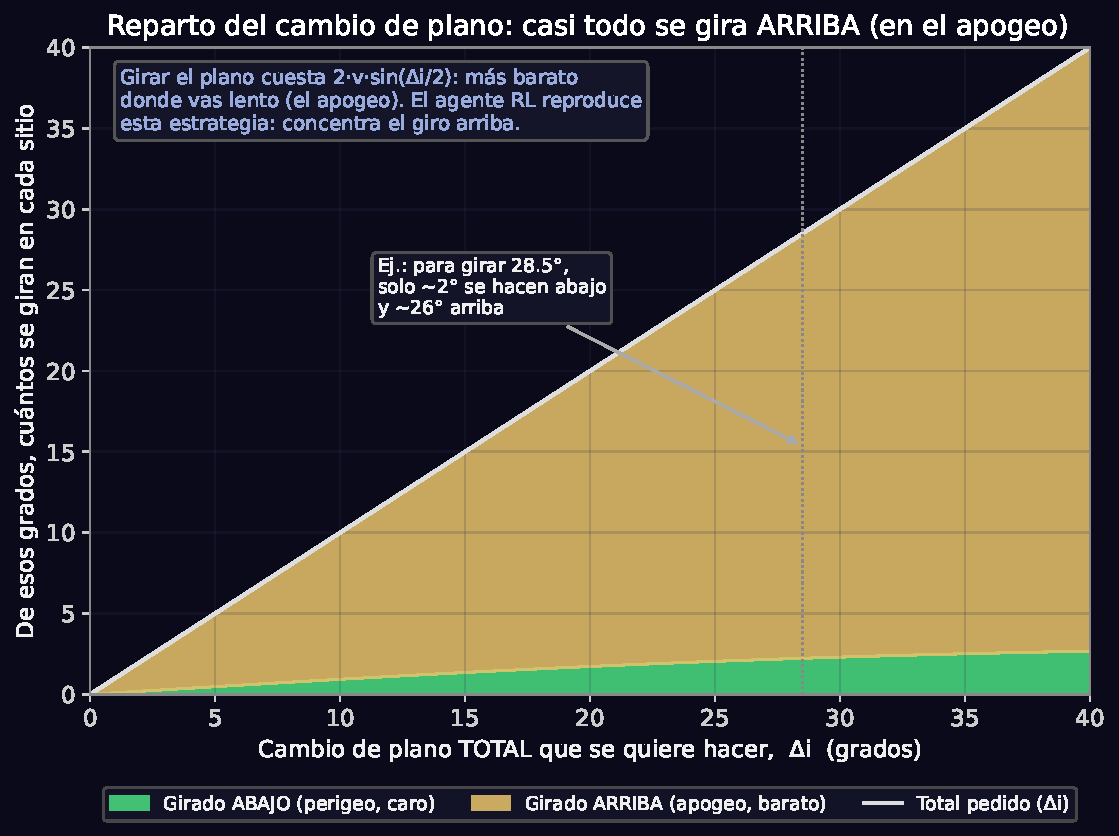
\includegraphics[width=0.82\textwidth]{tex/imagenes/ia_transfer3d_reparto.pdf}
  \caption{Reparto óptimo del cambio de plano entre los dos impulsos en función del giro total pedido $\Delta i$. Elaboración propia}
  \label{fig:ia3d-reparto}
\end{figure}

La Figura~\ref{fig:ia3d-orbita} representa en tres dimensiones una de estas maniobras (\gls{LEO}$\rightarrow$\gls{GEO} con $28{,}5^{\circ}$ de cambio de plano) ejecutada con los impulsos del agente: se aprecian la órbita inicial en el plano de referencia, la elipse de transferencia y la órbita final inclinada.

\begin{figure}[htbp]
  \centering
  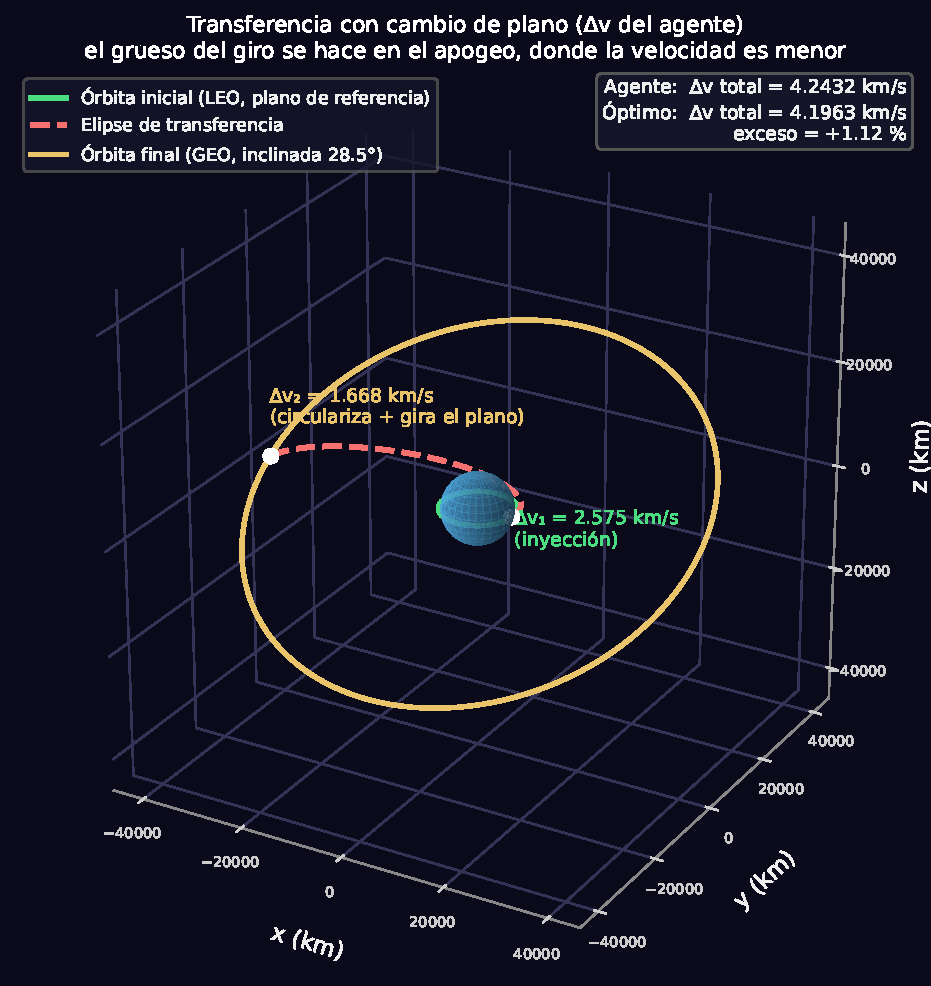
\includegraphics[width=0.72\textwidth]{tex/imagenes/ia_transfer3d_orbita.pdf}
  \caption{Transferencia \gls{LEO}$\rightarrow$\gls{GEO} con un cambio de plano de $28{,}5^{\circ}$ en tres dimensiones. Elaboración propia}
  \label{fig:ia3d-orbita}
\end{figure}

Por último, la invariancia de escala se conserva también en tres dimensiones (Figura~\ref{fig:ia3d-invariancia}): la misma política, aplicada sin reentrenar a los nueve cuerpos, produce el mismo exceso sobre el óptimo para cada par $(R,\Delta i)$. Un único agente resuelve, por tanto, las transferencias con cambio de plano en cualquier cuerpo, con un exceso inferior al $1{,}2\,\%$ en planetas como Marte o Júpiter, nunca vistos durante el entrenamiento.

\begin{figure}[htbp]
  \centering
  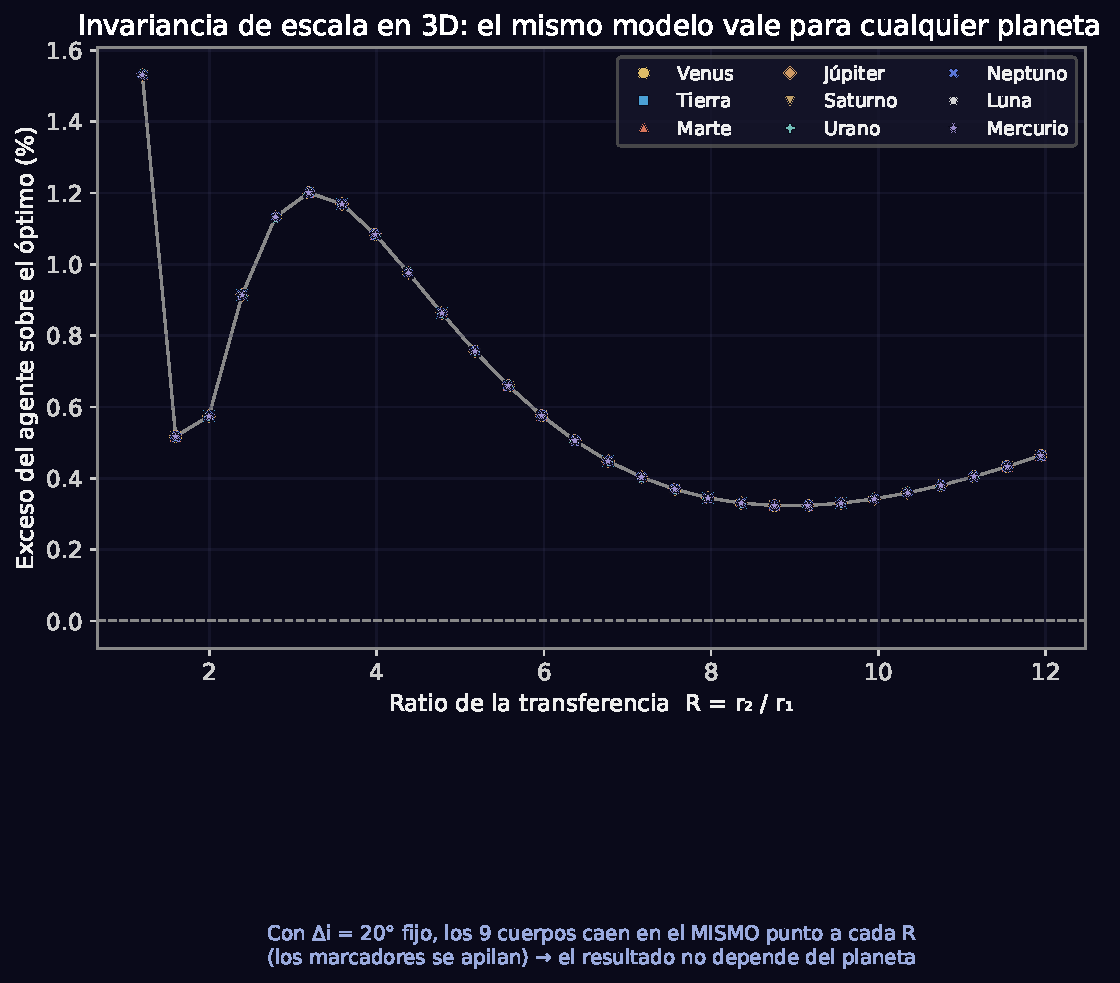
\includegraphics[width=0.82\textwidth]{tex/imagenes/ia_transfer3d_invariancia.pdf}
  \caption{Exceso del agente tridimensional sobre el óptimo al aplicar la misma política, sin reentrenar. Elaboración propia}
  \label{fig:ia3d-invariancia}
\end{figure}

\subsection{Aerofrenado multi-planeta: generalización y comportamiento emergente}
\label{sec:res-ia-aero}

El segundo agente, el de aerofrenado (Sección~\ref{sec:ia-aerofrenado}), se entrenó como un especialista por planeta para los siete cuerpos con atmósfera. Cada especialista no memoriza un caso concreto, sino que aprende la estrategia: probado en cincuenta escenarios aleatorios distintos por cuerpo ---con el apogeo inicial y la órbita objetivo sorteados---, los siete agentes los resuelven todos con éxito (50 de 50 en cada planeta), lo que demuestra que generalizan dentro de su cuerpo en lugar de aprender de memoria un caso. Las figuras individuales de cada cuerpo ---la comparación con la estrategia ingenua y la circularización de la órbita--- se recogen en el apéndice~\ref{ap:aero-planetas}, cuya consulta permite apreciar las diferencias de comportamiento entre unos planetas y otros.

La Figura~\ref{fig:ia-apogeo-pasada} muestra el descenso del apogeo pasada a pasada. En todos los cuerpos el apogeo decae de forma aproximadamente exponencial hasta la órbita objetivo, pero el número de pasadas necesarias varía mucho ---de poco más de un centenar en Marte a cerca de quinientas en Júpiter---, reflejo de lo distinta que es cada atmósfera.

\begin{figure}[htbp]
  \centering
  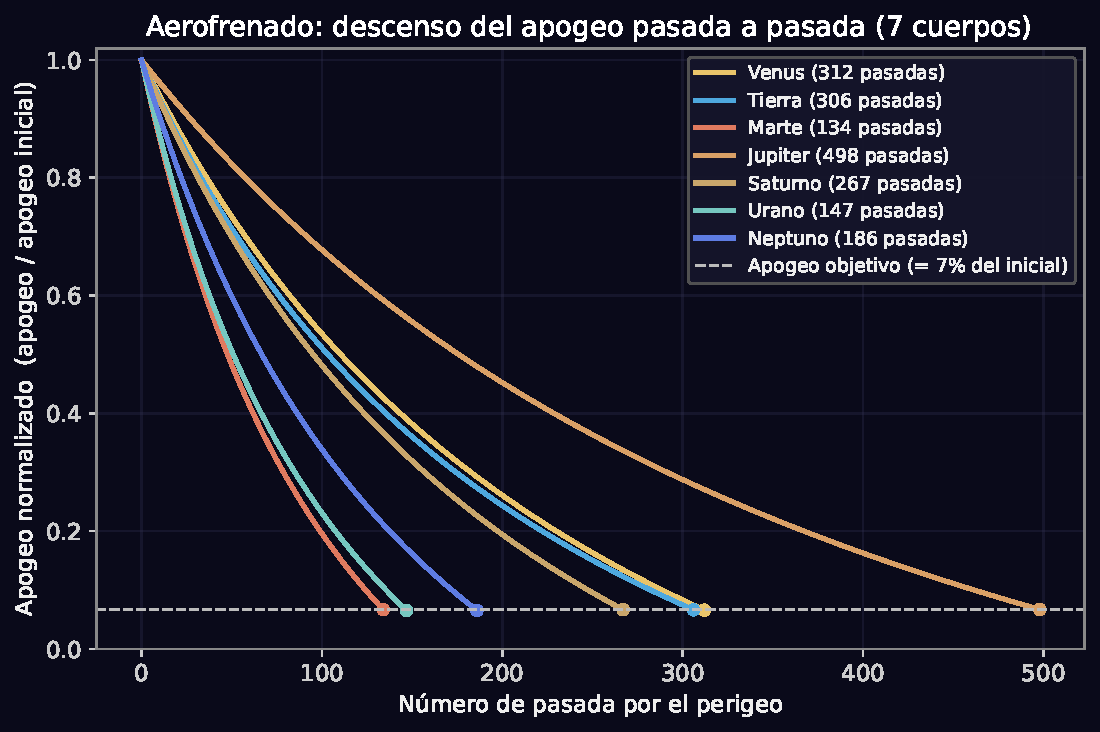
\includegraphics[width=0.82\textwidth]{tex/imagenes/ia_aero_apogeo_pasada.pdf}
  \caption{Descenso del apogeo (normalizado a su valor inicial) pasada a pasada para los siete cuerpos con atmósfera. Elaboración propia.}
  \label{fig:ia-apogeo-pasada}
\end{figure}

La Figura~\ref{fig:ia-orbita-aero} ilustra el mismo proceso desde otra perspectiva: para Marte, la órbita pasa de muy elíptica a prácticamente circular conforme su apogeo desciende pasada a pasada.

\begin{figure}[htbp]
  \centering
  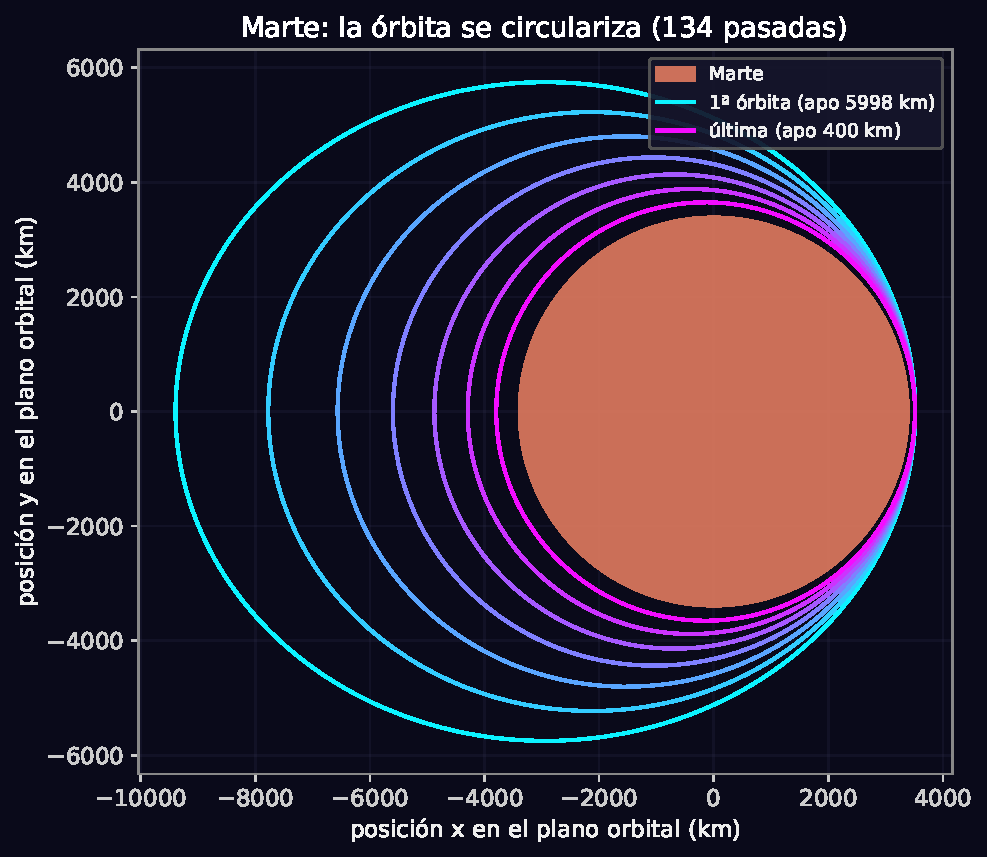
\includegraphics[width=0.62\textwidth]{tex/imagenes/ia_aero_orbita_marte.pdf}
  \caption{Aerofrenado en Marte. Elaboración propia}
  \label{fig:ia-orbita-aero}
\end{figure}

Que el agente aprende una verdadera estrategia, y no un comportamiento trivial, se aprecia al compararlo con una estrategia ingenua que mantiene el perigeo en un valor alto y seguro (Figura~\ref{fig:ia-vs-tonta}). El agente aprende a bajar el perigeo hasta apurar el frenado y alcanza el objetivo en una fracción de las pasadas; la estrategia ingenua, en cambio, frena tan despacio que no llega a completar la maniobra.

\begin{figure}[htbp]
  \centering
  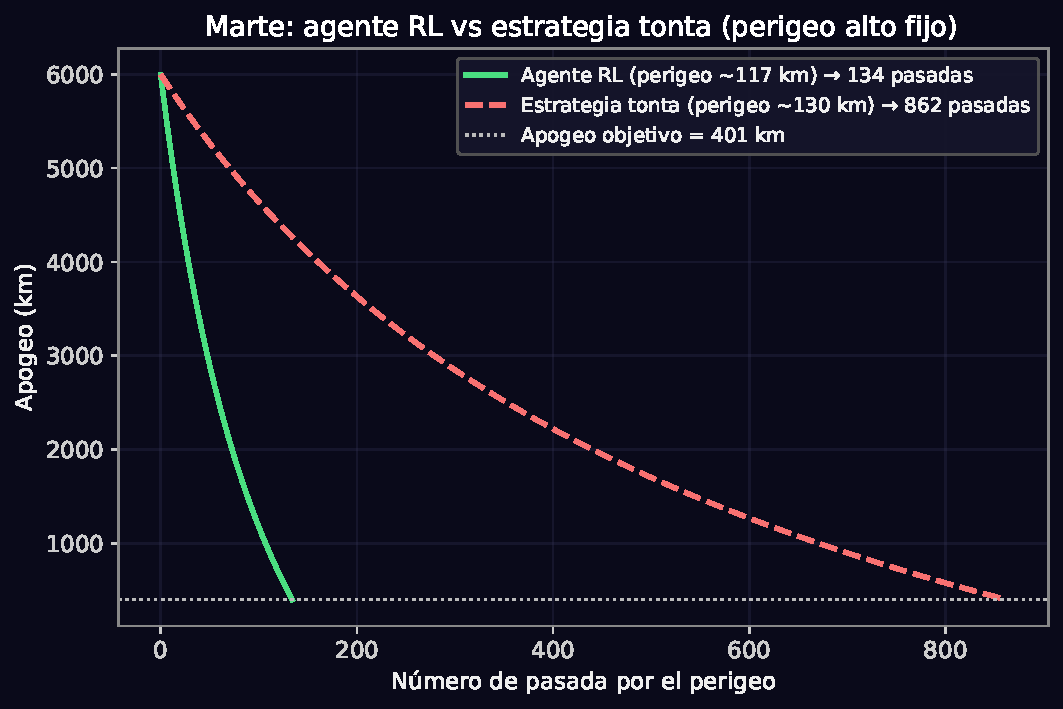
\includegraphics[width=0.82\textwidth]{tex/imagenes/ia_aero_vs_tonta_marte.pdf}
  \caption{Aerofrenado en Marte: agente de \gls{RL} frente a una estrategia ingenua de perigeo alto fijo. Elaboración propia}
  \label{fig:ia-vs-tonta}
\end{figure}

El resultado más interesante es emergente: el agente no busca el perigeo más bajo posible ---el crítico, en el que la presión dinámica~\eqref{eq:presion-dinamica} alcanzaría el límite---, sino el más bajo seguro, dejando un margen. La Figura~\ref{fig:ia-presion} compara la presión dinámica máxima a la que opera cada agente con el límite de la nave ($q_{\max}=0{,}6\ \mathrm{N/m^2}$). Ese margen no es uniforme: es amplio donde la atmósfera ya frena con eficacia (Urano, $q\approx 0{,}16\ \mathrm{N/m^2}$) y ajustado donde el agente necesita apurar para frenar lo suficiente (Júpiter, $q\approx 0{,}40\ \mathrm{N/m^2}$). Este equilibrio entre rapidez y seguridad no se programó: surge del aprendizaje.

\begin{figure}[htbp]
  \centering
  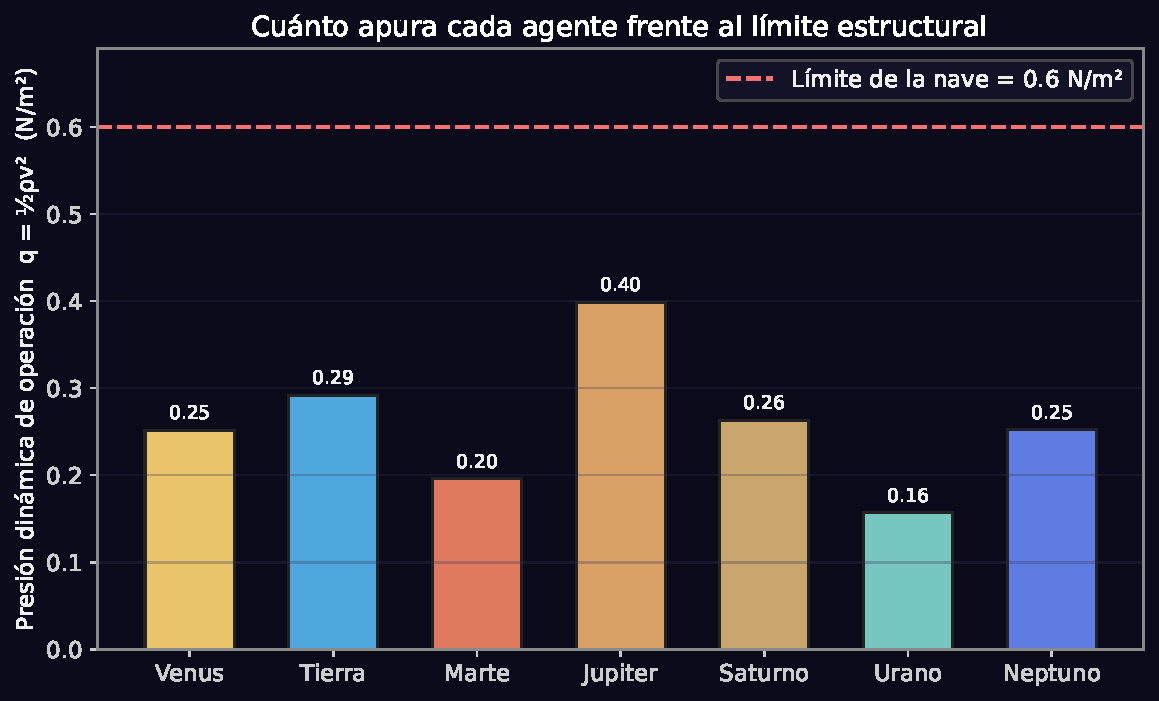
\includegraphics[width=0.82\textwidth]{tex/imagenes/ia_comp_presion.pdf}
  \caption{Presión dinámica máxima de operación de cada agente frente al límite de la nave ($q_{\max}=0,6N/m^2$). Elaboración propia.}
  \label{fig:ia-presion}
\end{figure}

Por último, la Figura~\ref{fig:ia-tiempo} traduce el número de pasadas a tiempo real (sumando los periodos orbitales): las campañas van de unas dos semanas (Marte) a unos tres meses (Júpiter). Estos tiempos son menores que los de las misiones reales de aerofrenado ---del orden de seis meses--- por dos supuestos del modelo ya discutidos: un coeficiente balístico inverso mayor (sección~\ref{sec:ia-aerofrenado}) y una órbita de captura más modesta. Júpiter merece una matización de honestidad: el aerofrenado resulta operable según el modelo de arrastre, pero inviable en la práctica por factores que el modelo no incluye, como la intensa radiación joviana y el calentamiento a las elevadísimas velocidades de paso por el perigeo.

\begin{figure}[htbp]
  \centering
  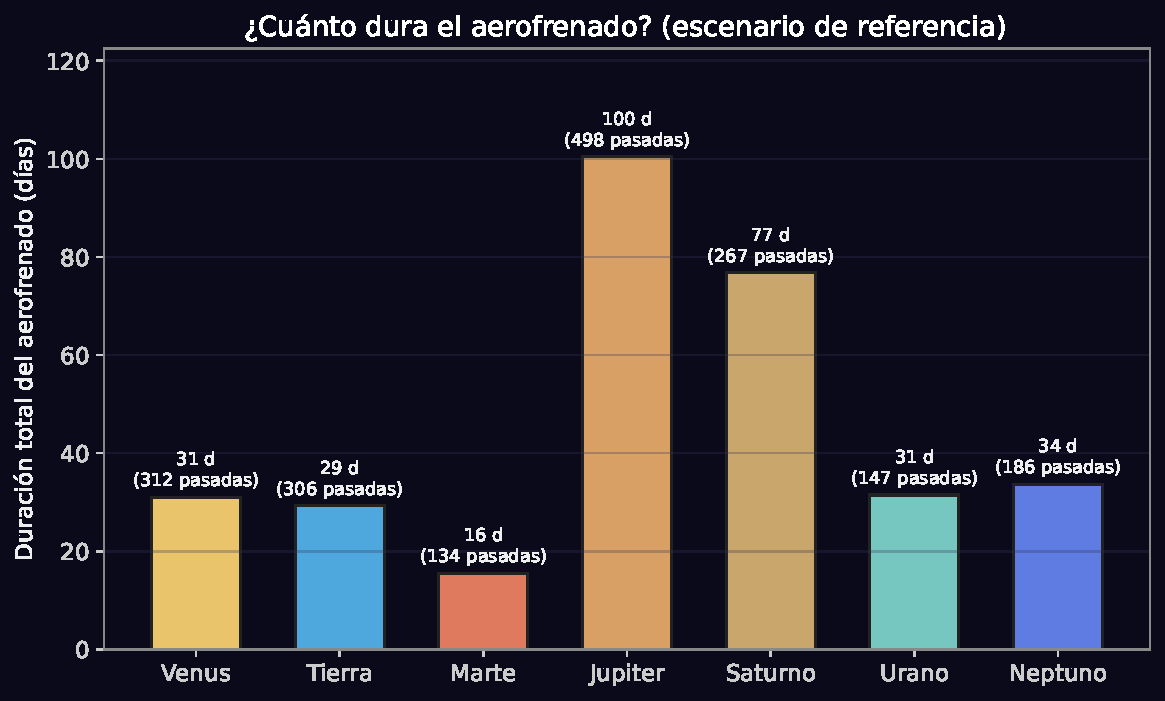
\includegraphics[width=0.82\textwidth]{tex/imagenes/ia_comp_tiempo.pdf}
  \caption{Duración total del aerofrenado (en días) y número de pasadas por cuerpo, en el escenario de referencia. Elaboración propia.}
  \label{fig:ia-tiempo}
\end{figure}

\subsection{Mantenimiento orbital: coste por cuerpo y aportación del aprendizaje}
\label{sec:res-ia-mantenimiento}

El quinto agente, el de mantenimiento orbital (Sección~\ref{sec:ia-mantenimiento}), se entrenó también como un especialista por planeta en los siete cuerpos con atmósfera. Probado en treinta órbitas aleatorias por cuerpo ---con la altitud y la inclinación sorteadas dentro de la franja operativa---, los siete agentes mantienen la órbita dentro de la banda durante toda la misión en los treinta escenarios de cada cuerpo. La Tabla~\ref{tab:res-keep} resume, para cada planeta, la franja de altitudes operativas, el coste anual de mantenimiento del agente y el de una estrategia ingenua de contraste.

\begin{table}[htbp]
  \centering
  \caption{Mantenimiento orbital por cuerpo.}
  \label{tab:res-keep}
  \begin{tabular}{lrrrr}
    \hline
    \textbf{Cuerpo} & \textbf{Franja} & {\boldmath $\Delta v$} \textbf{agente} & {\boldmath $\Delta v$} \textbf{ingenua} & \textbf{Ahorro} \\
     & \textbf{(km)} & \textbf{(m/s/año)} & \textbf{(m/s/año)} & \\
    \hline
    Venus   & 263--436    & 80,1 & 90,7  & 11,7\,\% \\
    Tierra  & 289--591    & 67,2 & 72,1  & 6,8\,\%  \\
    Marte   & 155--206    & 77,1 & 144,4 & 46,6\,\% \\
    Júpiter & 1524--2247  & 80,3 & 82,0  & 2,1\,\%  \\
    Saturno & 1969--3206  & 84,8 & 85,7  & 1,1\,\%  \\
    Urano   & 4899--7008  & 69,7 & 69,6  & $-0{,}1$\,\% \\
    Neptuno & 2111--3513  & 80,3 & 80,6  & 0,4\,\%  \\
    \hline
  \end{tabular}
\end{table}

La franja operativa de cada cuerpo no se fija a mano, sino que se deriva de su atmósfera (Figura~\ref{fig:keep-franjas}): comprende las altitudes en las que el mantenimiento cuesta 2 y 250 m/s al año. Así, mientras en Marte la franja queda en torno a los 150--200 km, en un gigante como Urano se sitúa por encima de los 4\,000 km, reflejo de lo extensa que es su atmósfera.

\begin{figure}[htbp]
  \centering
  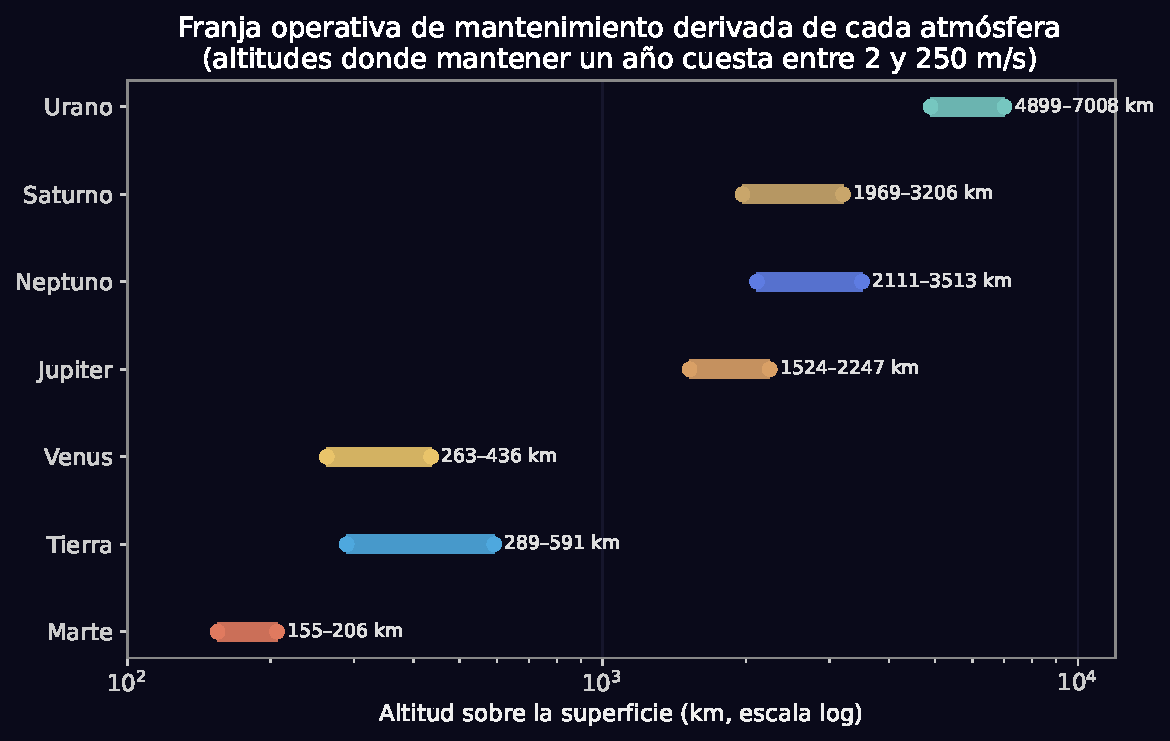
\includegraphics[width=0.82\textwidth]{tex/imagenes/ia_keep_franjas.pdf}
  \caption{Franja de altitudes operativas de cada cuerpo en escala logarítmica. Elaboración propia.}
  \label{fig:keep-franjas}
\end{figure}

El coste de mantenimiento cae de forma acusada con la altitud (Figura~\ref{fig:keep-coste}), reflejo directo del descenso casi exponencial de la densidad atmosférica: mantener una órbita en el borde inferior de la franja puede costar más de cien veces lo que cuesta una en el borde superior. Es la razón física de que volar bajo resulte tan ``caro'' en combustible.

\begin{figure}[htbp]
  \centering
  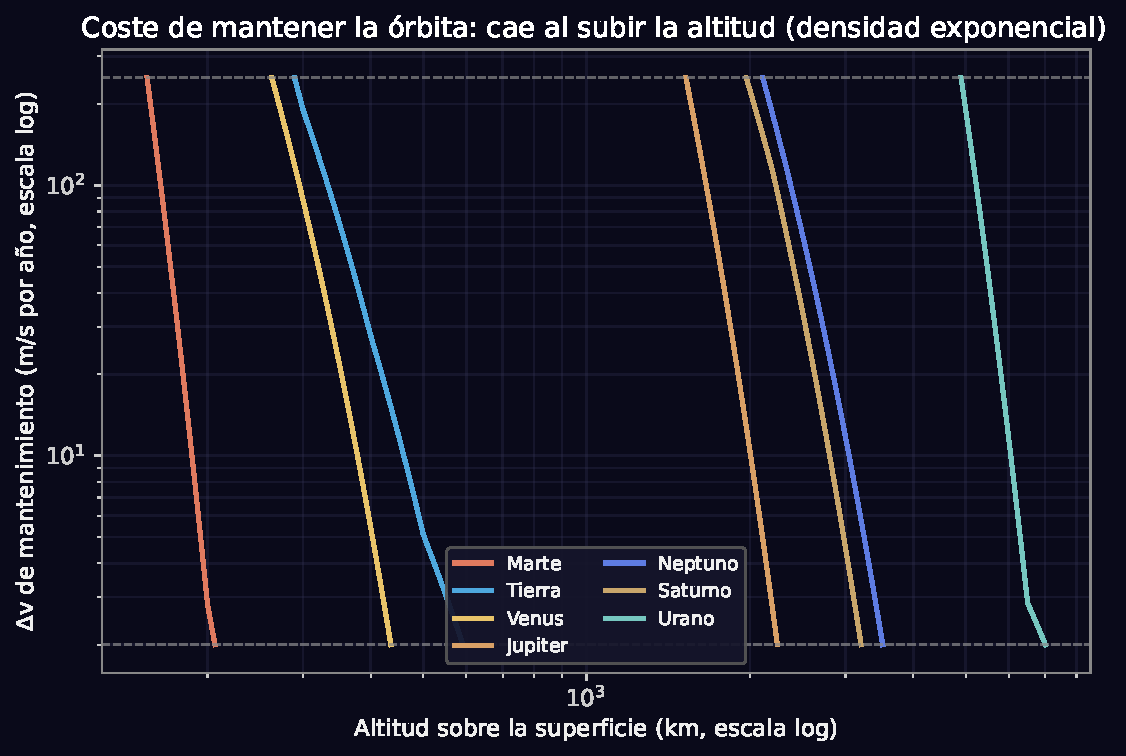
\includegraphics[width=0.82\textwidth]{tex/imagenes/ia_keep_coste_altitud.pdf}
  \caption{Coste anual de mantenimiento ($\Delta v$ por año) frente a la altitud. Elaboración propia.}
  \label{fig:keep-coste}
\end{figure}

El comportamiento del agente se aprecia en la Figura~\ref{fig:keep-diente}: frente a la estrategia ingenua, que deja caer la órbita y la sube de golpe describiendo un característico diente de sierra, el agente aprende a aplicar correcciones pequeñas y frecuentes que mantienen la altitud mucho más estable, cerca del objetivo. La banda sombreada es la tolerancia ($\pm$20 km).

\begin{figure}[htbp]
  \centering
  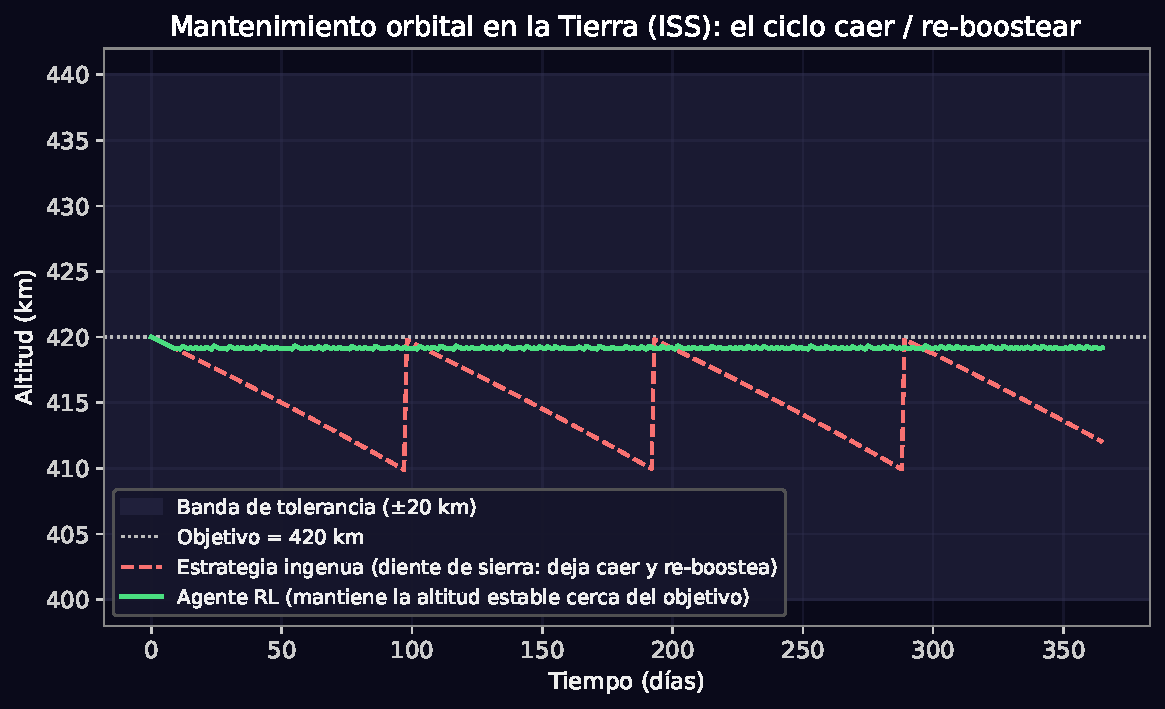
\includegraphics[width=0.82\textwidth]{tex/imagenes/ia_keep_diente_sierra.pdf}
  \caption{Mantenimiento de una órbita tipo \gls{ISS} (420 km). Elaboración propia.}
  \label{fig:keep-diente}
\end{figure}

La aportación del aprendizaje depende del régimen (Figura~\ref{fig:keep-ahorro}). El $\Delta v$ de mantenimiento está casi enteramente fijado por la física ---es el que repone la energía que el rozamiento sustrae---, de modo que el agente no puede ahorrar combustible más allá de ese mínimo. Donde sí marca diferencia es allí donde el control fino importa: en Marte, cuya atmósfera tiene una altura de escala pequeña y una franja estrecha, el agente ahorra cerca del 45\,\% frente a la estrategia ingenua; en los planetas gigantes, en cambio, la dinámica es lenta y suave, la heurística sencilla ya es casi óptima y el margen se reduce a un uno o dos por ciento. El agente nunca es peor que la heurística: la iguala donde la física fija el coste y la supera con claridad donde hay margen para un control más hábil.

\begin{figure}[htbp]
  \centering
  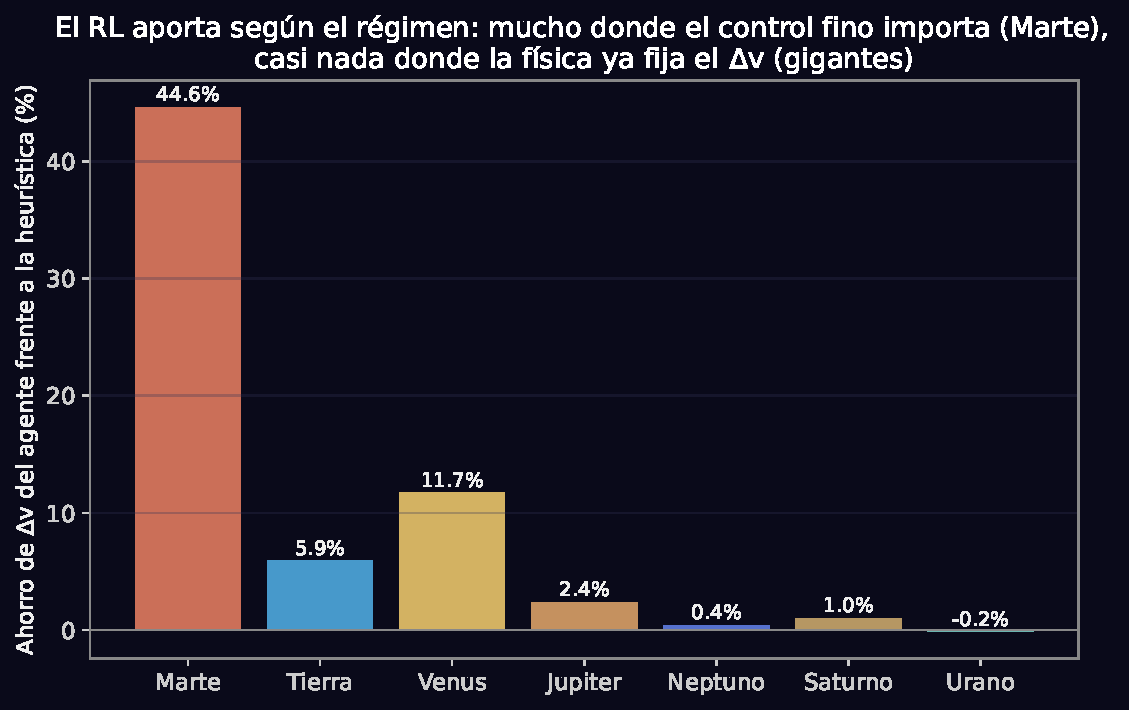
\includegraphics[width=0.82\textwidth]{tex/imagenes/ia_keep_ahorro.pdf}
  \caption{Ahorro de combustible del agente frente a la estrategia ingenua, por cuerpo. Elaboración propia.}
  \label{fig:keep-ahorro}
\end{figure}

En conjunto, el valor de este agente no reside tanto en el ahorro de combustible ---acotado por la física--- como en la generalización: una misma formulación, con la física derivada de cada atmósfera, mantiene órbitas operativas en los siete cuerpos con atmósfera. La precesión del plano por $J_2$, que el agente contabiliza pero no corrige, alcanza varios miles de grados al año en las órbitas bajas estudiadas ---del orden de $-5^\circ$ al día para una órbita tipo \gls{ISS}, en consonancia con la regresión nodal real de la estación---, lo que ilustra por qué combatirla resultaría prohibitivo.

\subsection{La capa de orquestación en funcionamiento}
\label{sec:res-ia-llm}

La capa de orquestación (Sección~\ref{sec:ia-llm}) integra los cinco agentes y los solvers clásicos en un único asistente conversacional. En la práctica, el usuario describe la maniobra en lenguaje natural y el asistente elige la herramienta adecuada, ejecuta el agente real y explica los números obtenidos, sin inventar ninguna cifra.

Los ejemplos que siguen son una selección; el apéndice~\ref{ap:llm-ejemplos} reúne conversaciones completas para cada tipo de maniobra ---cambio de plano, aerofrenado, viajes interplanetarios y \textit{porkchop}---, con la captura del diálogo y la figura que el asistente genera en cada caso, y merece la pena consultarlo para apreciar el alcance real del asistente.

La Figura~\ref{fig:llm-transferencia} muestra una interacción típica: ante la petición de subir a la órbita geoestacionaria, el asistente reconoce que se trata de una transferencia, invoca el agente correspondiente, recupera el $\Delta v$ real y lo contrasta con el óptimo de Hohmann. La Figura~\ref{fig:llm-mantenimiento} ilustra una consulta de mantenimiento orbital, resuelta con el agente del capítulo anterior: el asistente devuelve el coste anual de combustible y aclara, con los datos de la herramienta, que el margen frente a una estrategia sencilla es pequeño.

\begin{figure}[htbp]
  \centering
  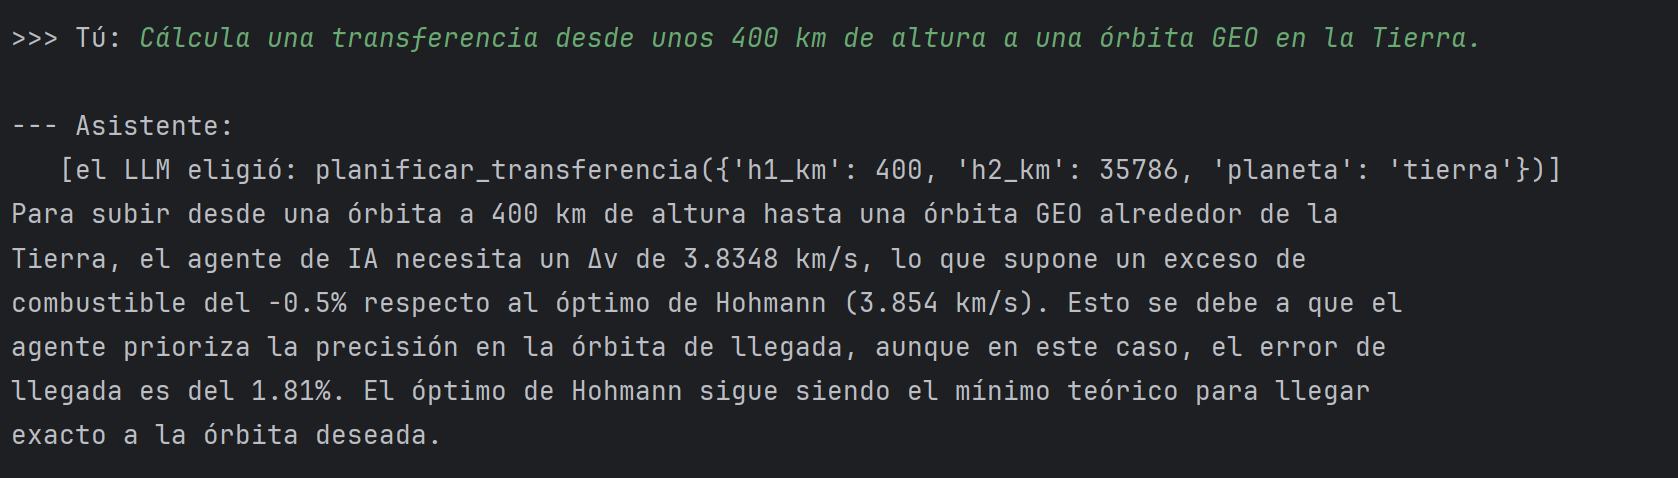
\includegraphics[width=0.9\textwidth]{tex/imagenes/llm_chat_transferencia.png}
  \caption{El asistente conversacional resolviendo una transferencia orbital. Elaboración propia.}
  \label{fig:llm-transferencia}
\end{figure}

\begin{figure}[htbp]
  \centering
  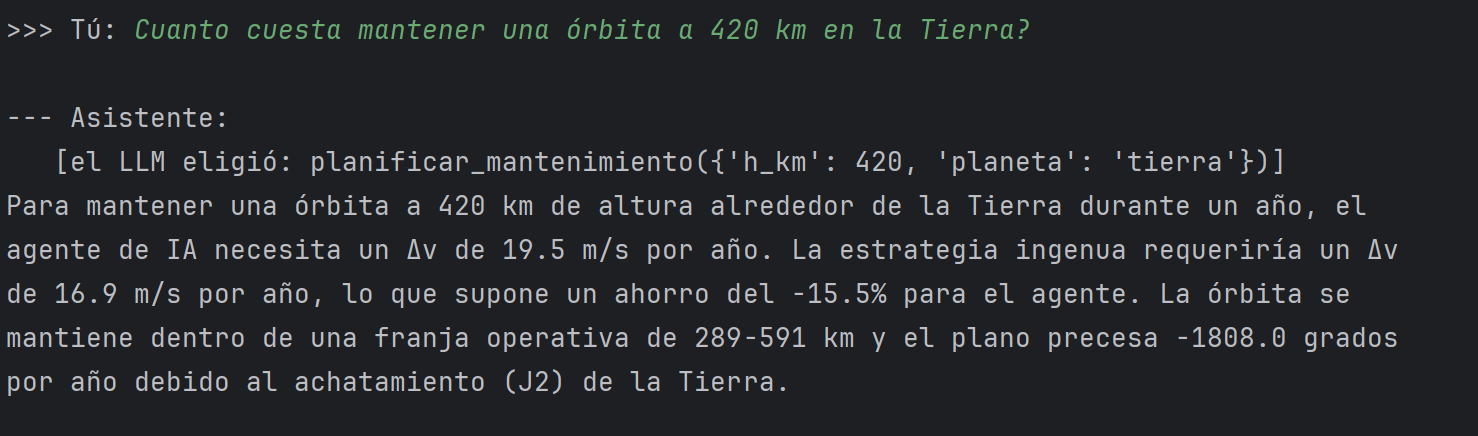
\includegraphics[width=0.9\textwidth]{tex/imagenes/llm_chat_mantenimiento.png}
  \caption{Consulta de mantenimiento orbital al asistente. Elaboración propia.}
  \label{fig:llm-mantenimiento}
\end{figure}

%\clearpage

El asistente conserva el contexto de la conversación. La Figura~\ref{fig:llm-memoria} recoge un turno en el que, tras haber consultado el mantenimiento en Marte, el usuario escribe simplemente ``ahora en Venus a 300 km''; el asistente recuerda que se hablaba de mantenimiento, elige por sí mismo la herramienta de dibujo y genera la figura, sin que el usuario tenga que repetir el tipo de maniobra.

\begin{figure}[htbp]
  \centering
  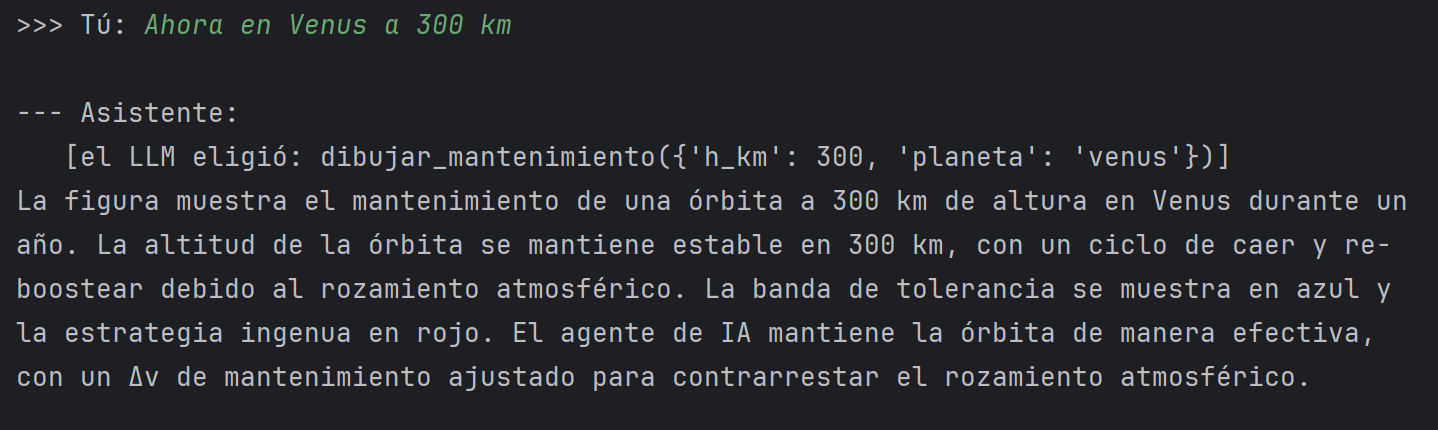
\includegraphics[width=0.9\textwidth]{tex/imagenes/llm_chat_mantenimiento_venus.png}
  \caption{Memoria conversacional. Elaboración propia.}
  \label{fig:llm-memoria}
\end{figure}

Las herramientas de dibujo permiten además producir figuras a la carta para la maniobra solicitada. La Figura~\ref{fig:llm-dientes} muestra dos ejemplos generados por el propio asistente ---el mantenimiento de una órbita a 170 km en Marte y a 300 km en Venus---, donde se aprecia el contraste entre el diente de sierra de la estrategia ingenua y la altitud estable que logra el agente. Ambas altitudes caen dentro de la franja operativa de su cuerpo; fuera de ella, sin arrastre apreciable, no habría nada que mantener (de ahí que, por ejemplo, una órbita a 300 km en Marte ---muy por encima de su franja--- no requiera correcciones).

\begin{figure}[htbp]
  \centering
  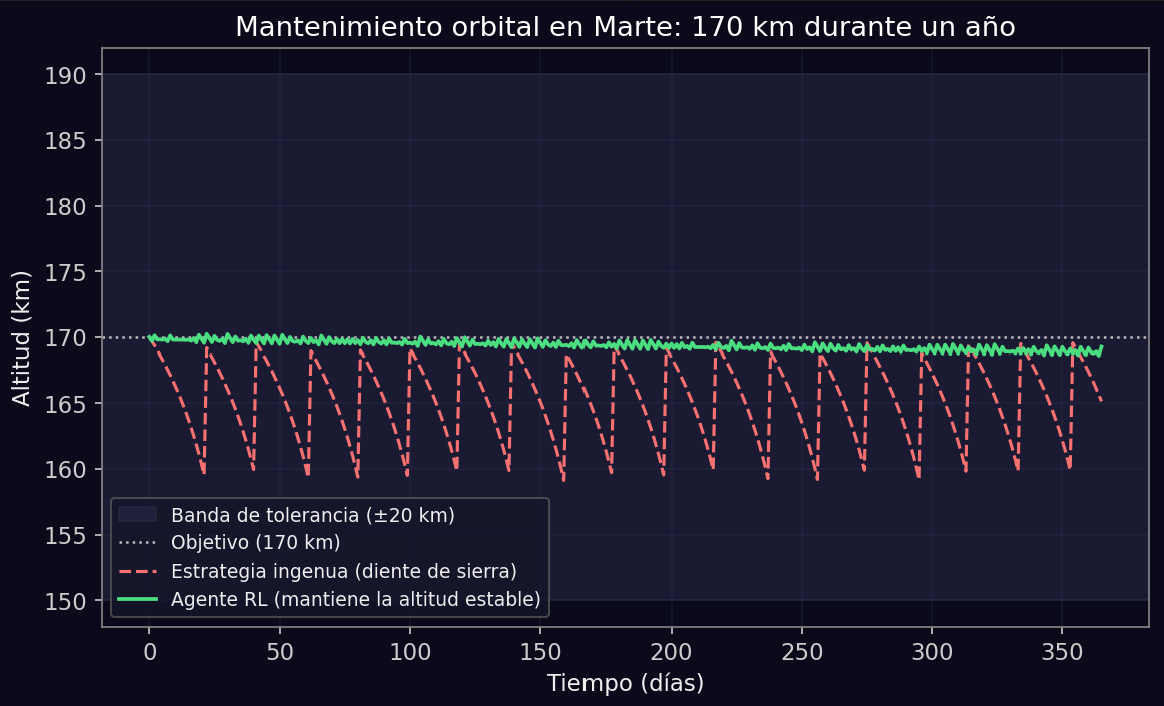
\includegraphics[width=0.78\textwidth]{tex/imagenes/mantenimiento_marte_dientes_sierra.png}\\[6pt]
  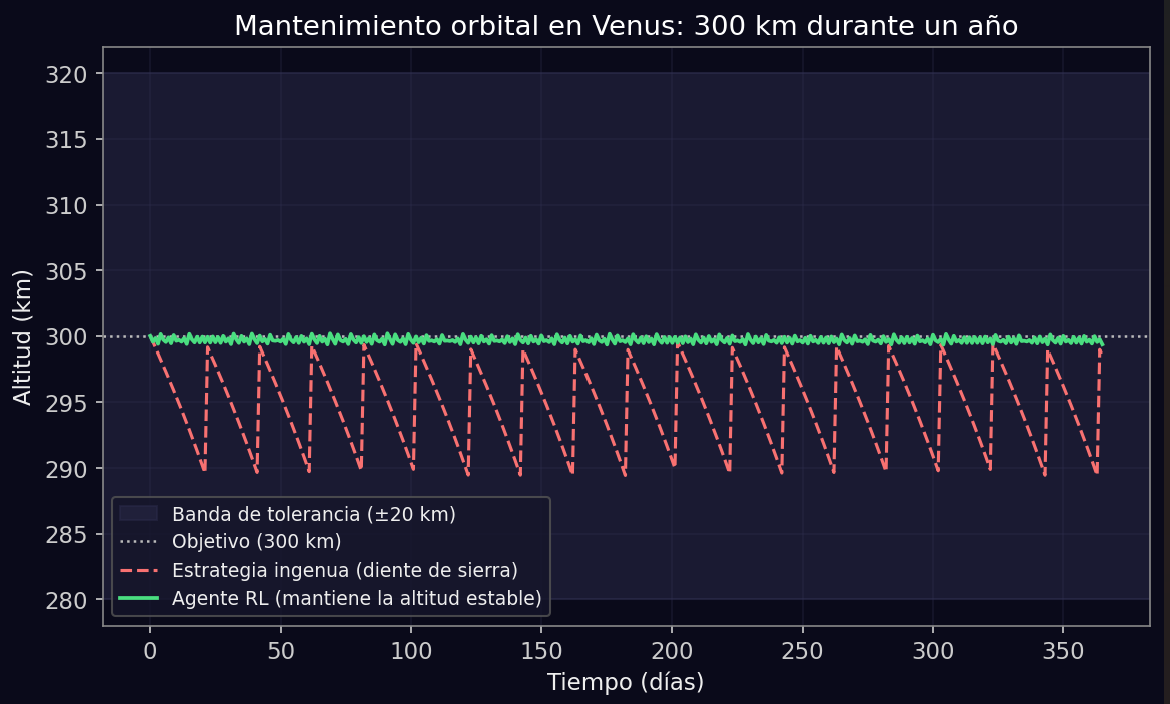
\includegraphics[width=0.78\textwidth]{tex/imagenes/mantenimiento_venus_dientes_sierra.png}
  \caption{Figuras generadas por el asistente a partir de peticiones en lenguaje natural. Elaboración propia.}
  \label{fig:llm-dientes}
\end{figure}

Más allá de los ejemplos, el comportamiento del asistente cumple las garantías de diseño: emplea solo cifras devueltas por las herramientas, encadena varias cuando hace falta (calcular y dibujar), recuerda el contexto de la conversación y declina las preguntas ajenas a la astrodinámica. Con ello, el sistema completo ---física validada, agentes de \gls{RL} y capa de orquestación--- queda integrado en una herramienta única, accesible en lenguaje natural.

\subsection{Evaluación cuantitativa de la capa de orquestación}
\label{sec:res-ia-llm-eval}

Para valorar el asistente más allá de ejemplos aislados, se preparó un banco de consultas anotadas que se ejecutan a través del orquestador real y se puntúan de forma sistemática. Cada consulta mide tres aspectos: si el \gls{LLM} elige la herramienta adecuada a la petición, si le pasa argumentos válidos (cuerpo, altitudes, fechas) y si las cifras de la respuesta proceden fielmente de las que devuelve la herramienta, sin datos inventados. La Tabla~\ref{tab:res-llm-eval} recoge el resultado sobre las veintitrés consultas de dominio, agrupadas por tipo de maniobra.

\begin{table}[htbp]
  \centering
  \caption{Evaluación de la capa de orquestación por categoría de consulta. Elaboración propia.}
  \label{tab:res-llm-eval}
  \begin{tabular}{lcccc}
    \hline\hline
    \textbf{Categoría} & \textbf{N} & \textbf{Herramienta} & \textbf{Argumentos} & \textbf{Cifras} \\
    \hline
    Transferencia   & 3 & 3/3 & 3/3 & 3/3 \\
    Cambio de plano & 2 & 2/2 & 2/2 & 2/2 \\
    Aerofrenado     & 3 & 3/3 & 3/3 & 3/3 \\
    Mantenimiento   & 3 & 3/3 & 3/3 & 3/3 \\
    Interplanetaria & 3 & 3/3 & 3/3 & 3/3 \\
    Porkchop        & 2 & 2/2 & 2/2 & 1/2 \\
    Dibujo          & 7 & 6/7 & 6/6 & 7/7 \\
    \hline
    \textbf{Total}           & \textbf{23} & \textbf{22/23} & \textbf{22/22} & \textbf{22/23} \\
    \hline\hline
  \end{tabular}
\end{table}

El asistente escogió la herramienta correcta en 22 de 23 consultas y empleó argumentos válidos en todas las que invocaron una herramienta. El único desajuste de selección se produjo ante una petición de dibujo deliberadamente ambigua ---``represéntame el viaje de la Tierra a Marte''---, en la que el modelo optó por la vista tridimensional interactiva en lugar de la bidimensional; ambas son representaciones válidas de la misma trayectoria. La fidelidad de las cifras fue igualmente alta: la respuesta se ancló a los datos de las herramientas en veintidós de las veintitrés consultas, y el único caso restante ---un \textit{porkchop}--- fue un falso positivo del verificador, que marcó como no respaldado el día de la fecha óptima que la propia herramienta había devuelto. En la práctica, ninguna respuesta introdujo números ajenos a los cálculos.

Se comprobó, por último, que el asistente declina las peticiones ajenas a la astrodinámica ---por ejemplo, preguntas de cultura general---, respondiendo con un rechazo en lugar de improvisar, en coherencia con el \textit{system prompt} acotado al dominio descrito en la sección~\ref{sec:ia-llm}. En conjunto, la evaluación confirma de forma cuantitativa las garantías de diseño de la capa de orquestación: selección acertada de la herramienta, argumentos correctos y respuestas ancladas a los cálculos reales.

\section{Contribuciones originales}
\label{sec:res-contribuciones}

Más allá del trabajo sistemático descrito en los capítulos anteriores, el desarrollo dio lugar a varias aportaciones originales -- metodológicas y de criterio--- que se recogen aquí de forma conjunta.

\subsection{Reconstrucción hidrostática de atmósferas sin datos in-situ}

Ni Urano ni Neptuno han sido sondeados in-situ: la \textit{Voyager}~2, única misión que los ha visitado, los sobrevoló (en 1986 y 1989) sin penetrar en su atmósfera. Los únicos datos provienen de la radio-ocultación: al ocultarse la sonda tras el planeta, su señal de radio atravesó la atmósfera y, de la refracción medida, se reconstruyeron perfiles de temperatura y presión. Esa técnica solo recupera estructura allí donde el gas es lo bastante denso para curvar la señal ---la troposfera y la estratosfera---, de ahí que no existan datos de la alta atmósfera ni medidas directas de densidad.

Para poder validar el modelo pese a esa carencia se desarrolló una reconstrucción del perfil de densidad por integración hidrostática. A partir de un reducido conjunto de puntos de referencia ---las anclas: pares de presión y temperatura tomados de los trabajos de Lindal~\cite{lindal1987,lindal1990,lindal1992}, como la tropopausa o el nivel de 1~bar--- se integra la ecuación del equilibrio hidrostático junto con la ley de los gases ideales (Sección~\ref{sec:hidrostatica}), obteniéndose un perfil de densidad continuo entre dichas anclas. Es, en esencia, el mismo procedimiento que emplean los modelos de referencia \gls{GRAM} de la \gls{NASA}.

El resultado se validó de forma cruzada contra esos mismos modelos (Uranus-\gls{GRAM} y Neptune \gls{GRAM}~\cite{uranusGRAM2021,neptuneGRAM2020}), con acuerdos inferiores al 2\,\%. Conviene acotar su alcance con honestidad: los datos de \textit{Voyager} llegan hasta unos 262~km en Urano y 300~km en Neptuno; por encima, el modelo extrapola apoyándose solo en  estimaciones de temperatura de la alta atmósfera~\cite{herbert1987,broadfoot1989}, por lo que sus capas superiores son las menos fiables. Aun con esa salvedad, una limitación de partida ---la ausencia de datos in-situ--- se convirtió en una aportación metodológica reutilizable.

\subsection{Detección y corrección de un error de calibración en Neptuno}

El modelo de capas incorpora un mecanismo de auto-comprobación: dado que la altura de escala $H$ de cada capa se deriva de la condición de continuidad, una $H$ que se aparte mucho de su valor físico $R_g T/(\bar{M} g)$ delata una densidad de referencia errónea. Este mecanismo reveló un error grave en el modelo preliminar de Neptuno ---una densidad de referencia unas cien veces demasiado baja, que producía desviaciones de hasta un factor 100---, que se corrigió reduciendo el factor de desviación típico de 8,0 a 1,2. Que la propia validación detecte errores capaces de invalidar toda simulación posterior es, en sí mismo, un resultado metodológico.

\subsection{Trazabilidad de datos: la lección de las IAs generalistas}

La norma de no aceptar ningún dato numérico sin contrastarlo con una fuente primaria ---adoptada tras detectar que unos valores de densidad de Júpiter procedentes de una \gls{IA} generalista erraban por un factor de hasta 2500 frente a la sonda Galileo (sección~\ref{sec:validacion-metodo})--- guió todo el trabajo. Esa trazabilidad sistemática, y la honestidad de documentar las limitaciones en lugar de ocultarlas, se consideran una aportación en sí mismas.

\subsection{Captura del acoplamiento arrastre--$J_2$}

En el caso de la \gls{ISS}, la regresión nodal simulada se desvía unos $0{,}8^\circ$ de la predicción de Brouwer, que no incluye arrastre. Lejos de ser un error, esa pequeña diferencia es un efecto físico real ---el acoplamiento arrastre--$J_2$: el arrastre reduce el semieje, lo que aumenta el movimiento medio y acelera la precesión--- que la simulación captura y la teoría de primer orden sin arrastre no puede reproducir (sección~\ref{sec:brouwer}). Reproducir ese efecto sutil es una muestra de la fidelidad del propagador.

\subsection{Detección automática de reentrada y fiabilidad de la pendiente}

Por último, el propagador detecta automáticamente la reentrada y, además, evalúa la fiabilidad de la pendiente de decaimiento mediante la razón entre el descenso secular y la amplitud de la oscilación periódica inducida por $J_2$: cuando esta última domina, advierte de que la tasa de decaimiento medida es poco fiable. Es una salvaguarda que evita extraer conclusiones de pendientes contaminadas por el bamboleo osculador.

\subsection{Generalización de maniobras por análisis dimensional}

La formulación de la transferencia impulsiva en variables adimensionales ---el ratio de radios $R$ y los impulsos medidos en unidades de la velocidad circular--- permite que un único agente, entrenado una sola vez, resuelva la maniobra en cualquier cuerpo del sistema solar sin reentrenamiento (Secciones~\ref{sec:ia-transfer} y~\ref{sec:res-ia-transfer}). Reconocer la invariancia de escala del problema y trasladarla al diseño del agente ---en lugar de entrenar un modelo por planeta--- es una aportación metodológica que convierte un problema aparentemente específico en uno universal. La misma idea se extiende a las transferencias con cambio de plano (Secciones~\ref{sec:ia-transfer3d} y~\ref{sec:res-ia-transfer3d}): basta añadir el ángulo de inclinación al estado adimensional para que un único agente resuelva también las maniobras tridimensionales en cualquier cuerpo.

\subsection{Criterio de aerofrenado por presión dinámica}

Para el aerofrenado se adoptó como límite de seguridad la presión dinámica $q=\tfrac{1}{2}\rho v^2$ ---el parámetro que controlan las campañas reales--- en lugar de una altitud fija (Sección~\ref{sec:ia-aerofrenado}). Calibrado con un valor realista, este criterio deriva automáticamente el corredor de perigeo seguro de cada planeta a partir de su propia atmósfera y se traslada de un cuerpo a otro, a diferencia de la densidad, que ignora el peso de la velocidad. De él emerge, además, un comportamiento no programado: el agente opera con un margen de seguridad que se ajusta a la eficacia frenante de cada atmósfera (Sección~\ref{sec:res-ia-aero}).

\subsection{Integración de física validada, aprendizaje y lenguaje natural}

La aportación que da unidad al conjunto es la integración, en un único sistema, de tres piezas que la revisión del estado del arte (Capítulo~\ref{ch:antecedentes}) encontraba siempre por separado: un modelo físico contrastado con datos de misión, unos agentes de \gls{RL} que generalizan las maniobras ---incluidas las que no admiten solución analítica--- y una capa de lenguaje natural que hace accesible todo el sistema.

Esa integración consta de una arquitectura híbrida: el aprendizaje se emplea solo donde aporta ---las maniobras con física incierta o sin fórmula---, mientras que los solucionadores clásicos se reservan para los problemas de óptimo conocido, sin forzar el aprendizaje allí donde una fórmula ya lo resuelve. Por encima de ambos, la capa basada en un \gls{LLM} orquesta las herramientas mediante el patrón de \textit{tool use} y explica los resultados anclándose de forma estricta a las cifras que estas devuelven, de modo que nunca inventa datos; se trata de una aplicación de los modelos de lenguaje a la planificación de maniobras que, según el propio estado del arte, es todavía incipiente.

Reunir estas capacidades ---y no cada una por separado, que ya existían--- es la contribución que responde a la laguna señalada en la Sección~\ref{sec:mot-resumen} (Tabla~\ref{tab:mot-comparativa}) y la que da sentido al trabajo en su conjunto.